\documentclass[table,aspectratio=169]{beamer}
%% Choose aspect ratio:
% [aspectratio=43]  % 4:3 (default)
% [aspectratio=169] % 16:9, wide

\usetheme[minimal, nofont, noheadline]{tugraz2018}
% \usetheme[iaik,]{tugraz2018}
%% Choose main theme variant:
% [standard]        % standard (default)
% [iaik]       % with institute's graphical acronym on the left
% [minimal]         % with reduced visuals

%% Choose your font style:
%                   % Helvetica (default for Corporate Design)
% [webfont]         % Source Sans Pro (as used on tugraz.at)
% [nofont]          % no font loaded - Computer Modern Sans

%% Choose your department's color instead of TU Graz tugred (optional):
% [arch]            % 
% [bau]             %
% [etit]            %
% [mbww]            %
% [tcvp]            %
% [mpug]            %
% [infbio]          %


\usepackage[utf8]{inputenc}
\usepackage[english]{babel}
%% Choose your language:
% [ngerman]   % German
% [english]   % English


%% Add your own packages, macros, etc.
\usepackage{xcolor,colortbl}
\usepackage{mathtools}
\usepackage{booktabs,nicematrix}
\usepackage{rotating}
\usepackage[style=alphabetic,backend=biber]{biblatex} % Bibliography
\addbibresource{\jobname.bib}                         % Bibliography
\usepackage{fontawesome}
\usepackage{filecontents}
\usepackage{setspace}
\usepackage{subcaption}
\usepackage{multirow}
\usepackage{bm}
\usepackage{pgfplots}
\usepackage[linesnumbered,ruled,vlined]{algorithm2e}
\usepackage{framed, color}
\usepackage{tikz}
\usetikzlibrary{external}
\usetikzlibrary{calc,patterns, arrows.meta, shapes.geometric, positioning, decorations.markings, decorations.pathmorphing}
\usetikzlibrary{cipher}
\usepackage{skinny}
\usepackage{tugcolors}
\usepackage{skinnyzero} % definitions for figures: colors, etc
\setbeamersize
{
	text margin left=0.4cm,
	text margin right=0.4cm
}

%% Enter presentation metadata
\title{Cryptanalysis Using Constraint Programming}
\author{Hosein Hadipour}
\date{TU Wien - Vienna, Austria}
%\institute{IAIK}
\instituteurl{hossein.hadipour@iaik.tugraz.at}

%% Logos
%\institutelogo{beamerthemetugraz/institute/IAIK}  % graphical acronym for [] theme (left margin)
% \additionallogo{figures/logo}  % additional institute/department logo (footline; optional)
% \logobar{Supported by: ...}  % sponsors (titlepage; optional)

%% Macros
\newcommand{\tikzmark}[1]{\tikz[overlay,remember picture] \node (#1) {};}

\colorlet{upper}{tugred}
\colorlet{upperfix}{tugyellow}
\colorlet{upperunknown}{upper}
\colorlet{lower}{tugblue}
%\colorlet{lower}{mach} % alternative, brighter tugblue
\colorlet{lowerfix}{tugmid}
\colorlet{lowerunknown}{lower}
\colorlet{common}{tuggreen}
\definecolor{gold}{HTML}{F0AB00}

\newcommand{\dllegupper}[1][black]{\legendwrap{\TFill[#1]{0,0}}}
\newcommand{\dlleglower}[1][black]{\legendwrap{\BFill[#1]{0,0}}}
\newcommand{\dllegend}{%
  \dllegupper[upperfix] active difference
  \dllegupper[upperunknown] unknown difference
  \dlleglower[lowerfix] active mask
  \dlleglower[lowerunknown] unknown mask%
}
\newcommand{\dlshortlegend}{%
  \dllegupper[upper] difference
  \dlleglower[lower] linear mask%
}
\newcommand{\dlfeistellegend}{%
  \tikz[stateopts,baseline=(base)]{\draw[upper,very thick] (0,0) -- (.7,0) ++(0,-.3) coordinate (base);} differential
  \tikz[stateopts,baseline=(base)]{\draw[lower,very thick] (0,0) -- (.7,0) ++(0,-.3) coordinate (base);} linear%
}

\newcolumntype{Y}{>{\centering\arraybackslash}X}
\newcommand{\smallmath}{\everydisplay{\fontsize{8pt}{10pt}\selectfont}}

% S-box tables
\newcommand{\ddt}{\texttt{DDT}\xspace}
\newcommand{\lat}{\texttt{LAT}\xspace}
\newcommand{\bct}{\texttt{BCT}\xspace}
\newcommand{\dlct}{\texttt{DLCT}\xspace}
\newcommand{\udlct}{\texttt{UDLCT}\xspace}
\newcommand{\ldlct}{\texttt{LDLCT}\xspace}
\newcommand{\edlct}{\texttt{EDLCT}\xspace}
\newcommand{\ddlct}{\texttt{DDLCT}\xspace}
% Correlation and probability
\newcommand{\corr}{\mathbb{C}\xspace}
\newcommand{\pr}{\mathbb{P}\xspace}
\newcommand{\corrmid}{\mathbb{R}\xspace}


% Distinguisher notations
\newcommand{\Up}{_{\textsc{u}}} % Suffix for upper part of the distinguisher
\newcommand{\Mid}{_{\textsc{m}}} % Suffix for middle part of the distinguisher
\newcommand{\Low}{_{\textsc{l}}} % Suffix for lower part of the distinguisher
\newcommand{\Dist}{_{\textsc{d}}} % Suffix to represent the distinguisher
\newcommand{\In}{_{\textrm{i}}} % Suffix for inputs
\newcommand{\Out}{_{\textrm{o}}} % Suffix for outputs
\newcommand{\MU}{_{\textsc{mu}}} % Suffix for middle part of the distinguisher
\newcommand{\ML}{_{\textsc{ml}}} % Suffix for middle part of the distinguisher

%%% commands to represent CSP/COP variables/constraints%%%
\newcommand{\ax}{\texttt{AX}\xspace} %AX
\newcommand{\ay}{\texttt{AY}\xspace} %AY
\newcommand{\az}{\texttt{AZ}\xspace} %AZ
\newcommand{\aw}{\texttt{AW}\xspace} %AW
\newcommand{\dx}{\texttt{DX}\xspace} %DX
\newcommand{\lx}{\texttt{LX}\xspace} %LX
\newcommand{\dy}{\texttt{DY}\xspace} %DY
\newcommand{\ly}{\texttt{LY}\xspace} %LY
\newcommand{\dz}{\texttt{DZ}\xspace} %DZ
\newcommand{\lz}{\texttt{LZ}\xspace} %LZ
\newcommand{\dw}{\texttt{DW}\xspace} %DW
\newcommand{\lw}{\texttt{LW}\xspace} %LW
\newcommand{\kx}{\texttt{KX}\xspace} %KX
\newcommand{\ky}{\texttt{KY}\xspace} %KY
\newcommand{\dtk}{\texttt{DTK}\xspace} %DTK
\newcommand{\dstk}{\texttt{DSTK}\xspace} %DSTK

\newcommand{\axu}{\texttt{AXU}\xspace} %AXU
\newcommand{\ayu}{\texttt{AYU}\xspace} %AYU
\newcommand{\azu}{\texttt{AZU}\xspace} %AZU
\newcommand{\dxu}{\texttt{DXU}\xspace} %DXU
\newcommand{\dxmu}{\texttt{DXMU}\xspace} %DXU
\newcommand{\dyu}{\texttt{DYU}\xspace} %DYU
\newcommand{\dzu}{\texttt{DZU}\xspace} %DZU
\newcommand{\lxu}{\texttt{LXU}\xspace} %LXU
\newcommand{\axl}{\texttt{AXL}\xspace} %AXL
\newcommand{\ayl}{\texttt{AYL}\xspace} %AYL
\newcommand{\azl}{\texttt{AZL}\xspace} %AZL
\newcommand{\dxl}{\texttt{DXL}\xspace} %DXL
\newcommand{\dxml}{\texttt{DXML}\xspace} %DXL
\newcommand{\dyl}{\texttt{DYL}\xspace} %DYL
\newcommand{\dzl}{\texttt{DZL}\xspace} %DZL
\newcommand{\lxl}{\texttt{LXL}\xspace} %LXL
\newcommand{\astk}{\texttt{ASTK}\xspace} %ASTK

\newcommand{\xu}{\texttt{XU}\xspace} %XU
\newcommand{\xl}{\texttt{XL}\xspace} %XL
\newcommand{\xmu}{\texttt{XMU}\xspace} %XMU
\newcommand{\xml}{\texttt{XML}\xspace} %XML
\newcommand{\PU}{\texttt{PU}\xspace} %XPU
\newcommand{\QL}{\texttt{QL}\xspace} %CL
\newcommand{\RM}{\texttt{RM}\xspace} %rm

\newcommand{\cp}[1]{\textit{\texttt{#1}}\xspace} % CP x
\newcommand{\csp}{\textit{\texttt{CSP}}\xspace} % CSP problem
\newcommand{\cop}{\textit{\texttt{COP}}\xspace} % COP problem
\newcommand{\cpmodel}{\mathcal{M}\xspace} % CP model M
\newcommand{\cpvars}{\mathcal{M}.\texttt{var}\xspace} % CP variables
\newcommand{\cpcons}{\mathcal{M}.\texttt{con}\xspace} % CP constraints
\newcommand{\cpobj}{\mathcal{M}.\texttt{obj}\xspace} % CP objective
\newcommand{\booltoint}{\textit{\texttt{bool2int}}\xspace} % CP bool2int operator
\newcommand{\cpif}{\textit{\texttt{if}}\xspace} % CP If
\newcommand{\cpthen}{\textit{\texttt{then}}\xspace} % CP Then
\newcommand{\cpelse}{\textit{\texttt{else}}\xspace} % CP Else
\newcommand{\cpelseif}{\textit{\texttt{elseif}}\xspace} % CP Elseif
\newcommand{\cpendif}{\textit{\texttt{endif}}\xspace} % CP Endif

\newcommand{\cplink}{\textit{\texttt{Link}}\xspace} % CP Link
\newcommand{\cpxor}{\textit{\texttt{XOR}}\xspace} % CP XOR
\newcommand{\cpsbox}{\textit{\texttt{S-box}}\xspace} % CP S-box
\newcommand{\cpmds}{\textit{\texttt{MDS}}\xspace} % CP MDS
\newcommand{\cpbranch}{\textit{\texttt{Branch}}\xspace} % CP Branching
\newcommand{\cpcopy}{\textit{\texttt{Copy}}\xspace} % Copy: equivalent to branching point
\newcommand{\cptrue}{\textit{\texttt{True}}\xspace} % CP True
\newcommand{\cpfalse}{\textit{\texttt{False}}\xspace} % CP False
\newcommand{\cplog}{\textit{\texttt{LG}}\xspace} % CP Log(g) - 0.53
\newcommand{\cpmax}{\textit{\texttt{max}}\xspace} % CP Max
\newcommand{\cpmin}{\textit{\texttt{min}}\xspace} % CP Min
\newcommand{\cpmdiff}{\textit{\texttt{Mdiff}}\xspace} % CP Mdiff
\newcommand{\cpminvdiff}{\textit{\texttt{Minvdiff}}\xspace} % CP Minvdiff
\newcommand{\cpmlin}{\textit{\texttt{Mlin}}\xspace} % CP Mlin
\newcommand{\cpminvlin}{\textit{\texttt{Minvlin}}\xspace} % CP Minvlin
\newcommand{\cpmdata}{\textit{\texttt{Mdata}}\xspace} % CP Mdata
\newcommand{\cpminvdata}{\textit{\texttt{Minvdata}}\xspace} % CP Minvdata

\makeatletter
\NewDocumentCommand{\DrawBox}{s O{}}{%
    \tikz[overlay,remember picture]{
    \IfBooleanTF{#1}{%
        \coordinate (RightPoint) at ($(left |- right)+(\linewidth-\labelsep-\labelwidth,0.0)$);
    }{%
        \coordinate (RightPoint) at (right.east);
    }%
    \draw[tugred,#2]
      ($(left)+(-0.2em,0.9em)$) rectangle
      ($(RightPoint)+(0.2em,-0.3em)$);}
}

\NewDocumentCommand{\DrawBoxWide}{s O{}}{%
    \tikz[overlay,remember picture]{
    \IfBooleanTF{#1}{%
        \coordinate (RightPoint) at ($(left |- right)+(\linewidth-\labelsep-\labelwidth,0.0)$);
    }{%
        \coordinate (RightPoint) at (right.east);
    }%
    \draw[tugred,#2]
      ($(left)+(-\labelwidth,0.9em)$) rectangle
      ($(RightPoint)+(0.2em,-0.3em)$);}
}

\newcommand{\sparen}{\vspace*{-.3cm}}
\newcommand<>\hlbox[2]{%
  \alt#3{\makebox[\dimexpr\width-2\fboxsep]{\colorbox{#1}{#2}}}{#2}%
}

\makeatother

\begin{document}

\begin{frame}[plain]
  \maketitle
\end{frame}

\section*{}
\begin{frame}{Outline}
  \tableofcontents
\end{frame}

%%%%%%%%%%%%%%%%%%%%%%%%%%%%%%%%%%%%%%%%%%%%%%%%%%%%%%%%%%%%%%%%%%%%%%%%
%%%%%%%%%%%%%%%%%%%%%%%%%%%%%%%%%%%%%%%%%%%%%%%%%%%%%%%%%%%%%%%%%%%%%%%%
\section{Background}
\sectionheader[\huge\color{tug}\faBook]{Background}

%%%%%%%%%%%%%%%%%%%%%%%%%%%%%%%%%%%%%%%%%%%%%%%%%%%%%%%%%%%%%%%%%%%%%%%%
\subsection{Constraint Programming (CP)}
% \sectionheader[\huge\color{tug}\faBook]{Constraint Programming}

\begin{frame}{Constraint Programming (CP)}
\begin{itemize}
% \item Programming in CP refers to the arrangement of a plan
% \item For example the \href{https://developers.google.com/optimization/scheduling/employee_scheduling}{employee scheduling problem}
\item Constraint Satisfaction/Optimization Problem (CSP/COP):
\begin{itemize}
\item We define a set of variables: $\mathcal{X} = \{\mathcal{X}_{1}, \ldots, \mathcal{X}_{n}\}$
\item We specify the domain of each variable: $\mathbb{F}_{2}, \mathbb{Z}, \mathbb{R}, \ldots$
\item We define a set of constraints: $\mathcal{C} = \{\mathcal{C}_{1}, \ldots, \mathcal{C}_{2}\}$
\item We define an objective function (if it is required)
\end{itemize}
\item Constraint Programming (CP): Searching for a solution for a CSP/COP
\item \textcolor{tugred}{MILP} and \textcolor{tugblue}{SAT} are special cases of CP
\end{itemize}
\end{frame}


%%%%%%%%%%%%%%%%%%%%%%%%%%%%%%%%%%%%%%%%%%%%%%%%%%%%%%%%%%%%%%%%%%%%%%%%
\begin{frame}[fragile]
\frametitle{Constraint Programming -- Example}
\begin{columns}
\column[c]{0.45\textwidth}
\begin{center}
\only<1>{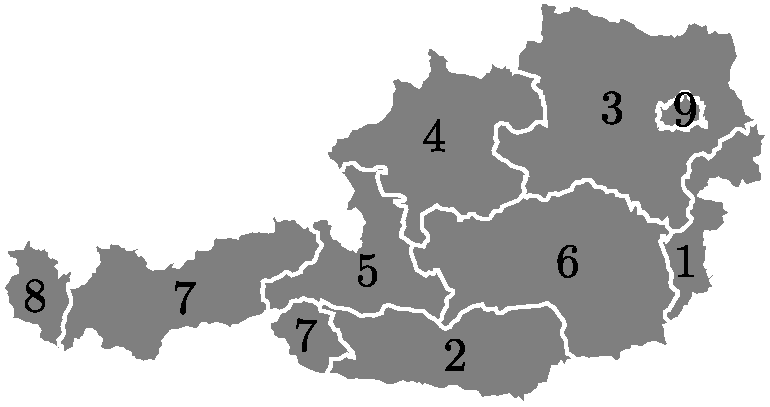
\includegraphics[width=0.9\textwidth]{./figures/austria.pdf}}
\only<2>{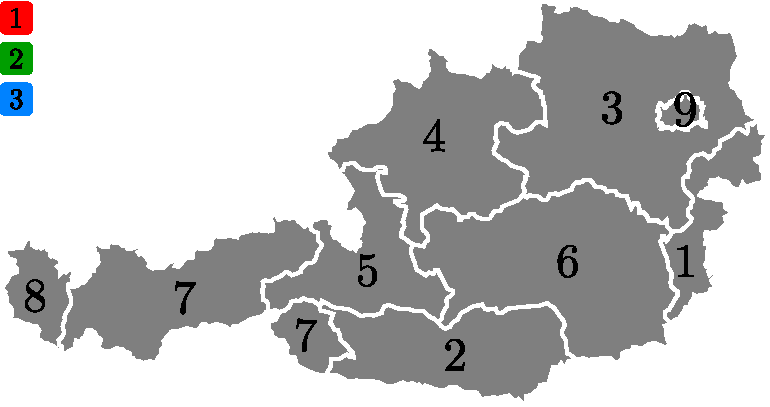
\includegraphics[width=0.9\textwidth]{./figures/austria_legend.pdf}}
\only<3>{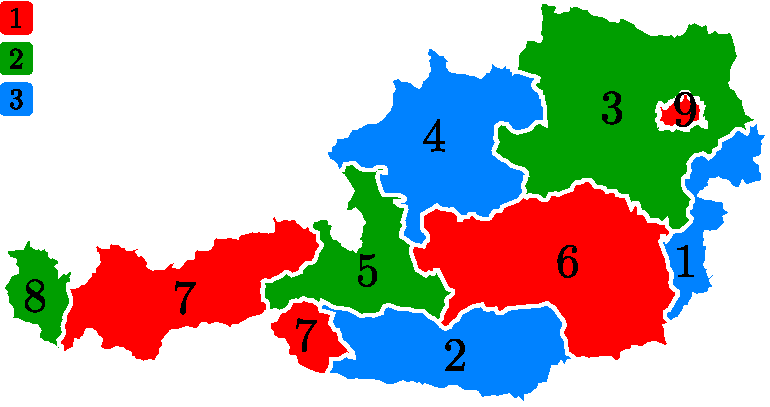
\includegraphics[width=0.9\textwidth]{./figures/austria3colored.pdf}}
\end{center}
\column[c]{0.55\textwidth}
\pause
{\scriptsize
\begin{verbatim}
int: nc = 3;
array[1..9] of var 1..nc: r;
constraint r[1] != r[3]; constraint r[1] != r[6];
constraint r[2] != r[5]; constraint r[2] != r[6]; 
constraint r[2] != r[7]; constraint r[3] != r[9]; 
constraint r[3] != r[6]; constraint r[3] != r[4];
constraint r[4] != r[6]; constraint r[4] != r[5];
constraint r[5] != r[6]; constraint r[5] != r[7];
constraint r[7] != r[8];
solve satisfy;
\end{verbatim}}
\pause
\vspace{-0.4cm}
{\scriptsize
\begin{verbatim}
r = [3, 3, 2, 3, 2, 1, 1, 2, 1];
\end{verbatim}}
\end{columns}
\end{frame}

%%%%%%%%%%%%%%%%%%%%%%%%%%%%%%%%%%%%%%%%%%%%%%%%%%%%%%%%%%%%%%%%%%%%%%%%
\subsection{Cryptanalysis}
% \sectionheader[\huge\color{tug}\faBook]{Cryptanalysis}

%%%%%%%%%%%%%%%%%%%%%%%%%%%%%%%%%%%%%%%%%%%%%%%%%%%%%%%%%%%%%%%%%%%%%%%%
\begin{frame}{Cryptanalysis}
\begin{itemize}
\item Complexity-theoretic approach (Public-Key primitives)
\item Cryptanalytic approach (Symmetric-Key primitives)
\onslide<2>{
\begin{itemize}
  \item \textcolor{tugred}{Differential attack} \cite{crypto_BihamS90} %(Full round DES \cite{crypto_BihamS92}/AES-256 \cite{crypto_BiryukovKN09})
  \item \textcolor{tugred}{Linear attack} \cite{eurocrypt_Matsui93} %(Full round DES \cite{eurocrypt_Matsui93}) 
  \item \textcolor{tugred}{Boomerang attack} \cite{fse_Wagner99} %(Full round COCONUT98 \cite{fse_Wagner99})
  \item \textcolor{tugred}{Differential-Linear attack} \cite{dl_crypto_LangfordH94} %(Full round COCONUT98 \cite{enhanced_dl_asiacrypt_BihamDK02})
  \item \textcolor{tugred}{Impossible-Differential attack} \cite{knudsen1998deal, eurocrypt_BihamBS99}
  \item \textcolor{tugred}{Integral attack} \cite{Lai1994, square_fse_DaemenKR97} %(Full-round \cipher{MISTY1}~\cite{crypto_Todo15})
  \item \textcolor{tugred}{Cube attack} \cite{eurocrypt_DinurS09} %(Best attack type on SHA-3 \cite{eurocrypt_HuangWXWZ17})
\end{itemize}
}
\end{itemize}
\end{frame}

%%%%%%%%%%%%%%%%%%%%%%%%%%%%%%%%%%%%%%%%%%%%%%%%%%%%%%%%%%%%%%%%%%%%%%%%
\begin{frame}{Automated Methods in Cryptanalysis}
Mounting cryptanalytic attacks against symmetric-key primitives:
\begin{itemize}
\item requires tracing the propagation of a certain property at the bit-level
\item implies solving a hard combinatorial optimization problem
\item is very time-consuming
\item is potentially an error-prone process
\end{itemize}
% \pause
\vspace{-0.4cm}
\begin{block}{Automated Methods in Cryptanalysis}
Getting the help or using of machines to \textcolor{tugred}{find}, \textcolor{tugblue}{build} or \textcolor{tuggreen}{optimize} the attacks
\end{block}
\end{frame}

%%%%%%%%%%%%%%%%%%%%%%%%%%%%%%%%%%%%%%%%%%%%%%%%%%%%%%%%%%%%%%%%%%%%%%%%
\begin{frame}{Different Approaches for Automatic Cryptanalysis}
\begin{itemize}
\item Dedicated algorithms
\item {\color<1>{tugred} Constraint Programming (CP)}
\begin{itemize}
\item {\color<1>{tugred} CP}
\item {\color<1>{tugred} MILP}
\item {\color<1>{tugred} SAT}
\item {\color<1>{tugred} SMT}
\end{itemize}
\item Artificial Intelligence (AI)
\end{itemize}
\end{frame}

% %%%%%%%%%%%%%%%%%%%%%%%%%%%%%%%%%%%%%%%%%%%%%%%%%%%%%%%%%%%%%%%%%%%%%%%%
% \subsection{A Basic Example}
% % \sectionheader[\huge\color{tug}\faBook]{Differential Analysis Using Constraint Programming}

% %%%%%%%%%%%%%%%%%%%%%%%%%%%%%%%%%%%%%%%%%%%%%%%%%%%%%%%%%%%%%%%%%%%%%%%%
% \begin{frame}{Differential Attack \cite{crypto_BihamS90}}
%   \vspace{-10pt}
%   \begin{columns}[onlytextwidth]
%     \column[c]{0.3\textwidth}
%     \scalebox{0.75}{
%       \begin{tikzpicture}[scale=0.5]
%         \foreach \i in {0,1,2,3}
%         \draw (0,-\i*4) rectangle ++(6,-2);
%         \foreach \i in {1,2,3}
%         \node[right] at (6,-\i*4+3) {$p_\i$};
%         \foreach \i in {0,1,2,3,4} {
%           \draw[->] (3,-\i*4+2) -- ++(0,-0.75);
%           \draw[<-] (3,-\i*4) -- ++(0,0.75);
%           \draw[<-] (3-0.25,-\i*4+1) -- ++(-1.25,0);
%           \node[left] at (1.5,-\i*4+1) {$K_\i$};          
%           \node[xor] at (3, -\i*4+1) {};
%         }
%         \node[right] at (4,1) {$\Delta_0$};
%         \node[right] at (4,-3) {$\Delta_1$};
%         \node[right] at (4,-7) {$\Delta_2$};
%         \node[right] at (4,-11) {$\Delta_3$};
%         \node[right] at (4,-15) {$\Delta_4$};
%         % \draw[->,very thick,tug] (6,1) -- ++(0,-12);
%         \path[->,tug,very thick,>=stealth] (6.5,1) edge[bend left]
%           node[rotate=270,above] {$\pr(\Delta_0 \rightarrow \Delta_3)$} ++(0,-12);
%         \path[->,tugblue,very thick,>=stealth] (6.5,-15) edge[bend right] 
%           node[font=\small,rotate=270,above] {guess $K_4$} ++(0,4);
%       \end{tikzpicture}
%     }
%     \column[c]{0.7\textwidth}    
%     \begin{enumerate}
%       \item Find ``good'' differential characteristic 
%         \[
%           \textcolor{tugred}{\Delta\In} = \Delta_0 \rightarrow \Delta_1 \rightarrow \Delta_2 \rightarrow \textcolor{tugred}{\Delta\Out} = \Delta_3
%         \]
%       \item Guess final key $K_4'$ and determine $\Delta_3'$
%         \medskip
%       \item The right key satisfies $\Delta_3' = \Delta_3$ with probability $\pr(\Delta_0 \rightarrow \Delta_3) = p_{1} \cdot p_{2} \cdot p_{3}$, while a wrong key satisfies $\Delta_3' = \Delta_3$ with probability $2^{-n}$
%         \medskip
%       \item \textit{Necessary condition} for the attack: $\pr \gg 2^{-n}$.
%         %, the attack will be faster than exhaustive key search
%     \end{enumerate}
%   \end{columns}
% \end{frame}


% %%%%%%%%%%%%%%%%%%%%%%%%%%%%%%%%%%%%%%%%%%%%%%%%%%%%%%%%%%%%%%%%%%%%%%%%
% \begin{frame}{A Simple Toy Block Cipher}
%   The block cipher $E_{k_0\|k_1}(m)$ encrypts 4 bits of plaintext using two 4-bit
%   keys:
%   \begin{align*}
%     c = E_{k_0\|k_1}(m) = \mathcal S(m \oplus k_0) \oplus k_1
%   \end{align*}

%   \begin{center}
%     \begin{tikzpicture}
%       \draw(0,0) node {$m$};
%       \draw[->](0.25,0) -- ++(0.5,0);
%       \node[xor] at (1, 0) (xor1) {};
%       \node[box, fill=tugblue] at (3, 0) (S) {\textcolor{white}{$S$}};
%       \draw[->](1.25,0) -- node[above] {$u$} (S);
%       \draw[->](S) -- node[above] {$v$} (4.75,0);
%       \node[xor] at (5, 0) (xor2) {};
%       \draw[->](5.25,0) -- ++(0.5,0);
%       \draw(6,0) node {$c$};
%       \draw[tug](1,1) node {$k_0$};
%       \draw[->](1,0.75) -- ++(0,-0.5);
%       \draw[tug](5,1) node {$k_1$};
%       \draw[->](5,0.75) -- ++(0,-0.5);
%     \end{tikzpicture}
%     \medskip

%     \setlength\extrarowheight{0.2ex} 
%     \scalebox{0.8}{
%       \begin{tabular}{@{}l*{16}{r}@{}}
%         \toprule
%         $x$                & 0 & 1 & 2 & 3 & 4 & 5 & 6 & 7 & 8 & 9 & a & b & c & d & e & f \\
%         \midrule
%         $\mathcal{S}  (x)$ & 4 & 0 & a & 7 & b & e & 1 & d & 9 & f & 6 & 8 & 5 & 2 & c & 3 \\
%         \bottomrule
%       \end{tabular}
%     }
%   \end{center}
%   \pause

%   Given $(m_0,c_0) = (\mathtt a,\mathtt 9)$ and $(m_1,c_1) = (\mathtt 5,\mathtt 6)$, what is the key?
%   \bigskip\pause

%   Brute force (exhaustive search): try all $2^4\cdot2^4=256$ keys.
% \end{frame}

% %%%%%%%%%%%%%%%%%%%%%%%%%%%%%%%%%%%%%%%%%%%%%%%%%%%%%%%%%%%%%%%%%%%%%%%%
% \begin{frame}{Differential Attack}
%   \vspace{-25pt}
%   \begin{center}
%     \scalebox{0.9}{
%     \begin{tikzpicture}
%       \draw(0,0) node {$m_0$};
%       \draw[->](0.25,0) -- ++(0.5,0);
%       % \draw(1,0) \xor{0.25};
%       \node[xor] at (1, 0) (xor1) {};
%       % \draw(3,0) node[primi, name=S] {$\mathcal S$} ++(-0.25,-0.25) rectangle ++(0.5,0.5);
%       \node[box, fill=tugblue] at (3, 0) (S) {\textcolor{white}{$S$}};
%       \draw[->](1.25,0) -- node[above] {$u_0$} (S);
%       \draw[->](S) -- node[above] {$v_0$} (4.75,0);
%       % \draw(5,0) \xor{0.25};
%       \node[xor] at (5, 0) (xor2) {};
%       \draw[->](5.25,0) -- ++(0.5,0);
%       \draw(6,0) node {$c_0$};

%       \draw[tug](1,0.75) node {$k_0$};
%       \draw[->](1,0.5) -- ++(0,-0.25);
%       \draw[tug](5,0.75) node {$k_1$};
%       \draw[->](5,0.5) -- ++(0,-0.25);

%       \begin{scope}[shift={++(0,-1.25)}]
%         \draw(0,0) node {$m_1$};
%         \draw[->](0.25,0) -- ++(0.5,0);
%         % \draw(1,0) \xor{0.25};
%         \node[xor] at (1, 0) (xor1) {};
%         % \draw(3,0) node[primi, name=S] {$\mathcal S$} ++(-0.25,-0.25) rectangle ++(0.5,0.5);
%         \node[box, fill=tugblue] at (3, 0) (S) {\textcolor{white}{$S$}};
%         \draw[->](1.25,0) -- node[above] {$u_1$} (S);
%         \draw[->](S) -- node[above] {$v_1$} (4.75,0);
%         % \draw(5,0) \xor{0.25};
%         \node[xor] at (5, 0) (xor2) {};
%         \draw[->](5.25,0) -- ++(0.5,0);
%         \draw(6,0) node {$c_1$};

%         \draw[tug](1,0.75) node {$k_0$};
%         \draw[->](1,0.5) -- ++(0,-0.25);
%         \draw[tug](5,0.75) node {$k_1$};
%         \draw[->](5,0.5) -- ++(0,-0.25);
%       \end{scope}
%       \draw[tugblue,thick](2,-2) node {?};
%       \draw[tugblue,thick,->](0,-2) -- (1.8,-2);
%       \draw[tugblue,thick,->](6,-2) -- (2.2,-2);
%     \end{tikzpicture}
%     }
%   \end{center}
%   \vspace{-0.5cm}
%   %\begin{block}
%   \emph{Strategy:}
%   \begin{enumerate}
%     \small
%     \item compute $\Delta\In = u_0 \oplus u_1$
%     \item guess $k_1$ (iterate over all values)
%       %\item compute $v_0' = c_0 \oplus k_1'$ and $v_1' = c_1 \oplus k_1'$
%     \item compute $u_0' = \mathcal S^{-1}(c_0 \oplus k_1')$ and $u_1' = \mathcal S^{-1}(c_1 \oplus k_1')$
%     \item check if $u_0 \oplus u_1 = u_0' \oplus u_1'$
%     \item if not: key guess was definitely wrong! (filtering)
%   \end{enumerate}
%   %\end{block}
% \end{frame}

%%%%%%%%%%%%%%%%%%%%%%%%%%%%%%%%%%%%%%%%%%%%%%%%%%%%%%%%%%%%%%%%%%%%%%%%
%%%%%%%%%%%%%%%%%%%%%%%%%%%%%%%%%%%%%%%%%%%%%%%%%%%%%%%%%%%%%%%%%%%%%%%%
\section{Autoguess}
\sectionheader[\huge\color{tug}\faBook]{Autoguess}

%%%%%%%%%%%%%%%%%%%%%%%%%%%%%%%%%%%%%%%%%%%%%%%%%%%%%%%%%%%%%%%%%%%%%%%%
\subsection{Guess-and-Determine (GD)}
% \sectionheader[\huge\color{tug}\faBook]{Guess-and-Determine (GD)}

%%%%%%%%%%%%%%%%%%%%%%%%%%%%%%%%%%%%%%%%%%%%%%%%%%%%%%%%%%%%%%%%%%%%%%%%
\begin{frame}{Guess-and-Determine (GD)}
  \vspace{-0.2cm}
  \begin{block}{Guess-and-Determine}
  \small
  Given a set of variables and a set of relations between them, 
  find the smallest subset of variables guessing the value of which 
  uniquely determines the value of the remaining variables.
  \end{block}
  % Start an animation
  % frame 1
  \only<2>{%
  \begin{example}
  \footnotesize
  \begin{columns}
  \column{0.40\textwidth}
  \begin{itemize}
  \footnotesize
  \item[\faCheckCircleO] $u, \ldots, z \in \mathbb{F}_{2}^{32}$
  \item[\faCheckCircleO] $F, G, H$: bijective functions
  \item[\faCheckCircleO]  $c_{1}, \ldots, c_{5}$: constants
  \end{itemize}
  \column{0.60\textwidth}
  \begin{align*}
  \left \{ \begin{array}{lr}
  F(u + v) \oplus G(x) \oplus y \oplus (z \lll 7) &= c_{1}\\
  G(u \oplus w) + (y \lll 3) + z &= c_{2}\\
  F(w \oplus x) + y \oplus z &= c_{3}\\
  F(u) \oplus G(w + z) &= c_{4}\\
  \left(F(u) \times G(w\lll 7)\right) + H(z\oplus v) &= c_{5}\\
  \end{array} \right.
  \end{align*}
  \end{columns}
  \end{example}
  }
  % frame 2
  \only<3>{%
  \begin{example}
  \footnotesize
  \begin{columns}
  \column{0.40\textwidth}
  \begin{itemize}
  \footnotesize
  \item[\faCheckCircle] Guess $\textcolor{tugred}{w}, \textcolor{tugred}{z}$
  \item[\faCheckCircle] Determine $\textcolor{tugblue}{u}~(4), \textcolor{tugblue}{y}~(2)$
  \item[\faCheckCircle] Determine $\textcolor{tugblue}{x}~(3), \textcolor{tugblue}{v}~(5)$
  \end{itemize}
  \column{0.60\textwidth}
  \begin{align*}
  \left \{ \begin{array}{lr}
  F(\textcolor{tugblue}{u} + \textcolor{tugblue}{v}) \oplus G(\textcolor{tugblue}{x}) \oplus \textcolor{tugblue}{y} \oplus (\textcolor{tugred}{z} \lll 7) &= c_{1}\\
  G(\textcolor{tugblue}{u} \oplus \textcolor{tugred}{w}) + (\textcolor{tugblue}{y} \lll 3) + \textcolor{tugred}{z} &= c_{2}\\
  F(\textcolor{tugred}{w} \oplus \textcolor{tugblue}{x}) + \textcolor{tugblue}{y} \oplus \textcolor{tugred}{z} &= c_{3}\\
  F(\textcolor{tugblue}{u}) \oplus G(\textcolor{tugred}{w} + \textcolor{tugred}{z}) &= c_{4}\\
  \left(F(\textcolor{tugblue}{u}) \times G(\textcolor{tugred}{w}\lll 7)\right) + H(\textcolor{tugred}{z}\oplus \textcolor{tugblue}{v}) &= c_{5}\\
  \end{array} \right.
  \end{align*}
  \end{columns}
  \end{example}
  }
\end{frame}

%%%%%%%%%%%%%%%%%%%%%%%%%%%%%%%%%%%%%%%%%%%%%%%%%%%%%%%%%%%%%%%%%%%%%%%%
\begin{frame}{Symmetric and Implication Relations}
  Assumption: Relations are symmetric or implication
  \begin{itemize}
    \item[\faCheckCircle] \textbf{Implication relations}:
    $\textcolor{tugred}{x_{1}, \ldots, x_{n} \Rightarrow y}$

    \item[\faCheckCircle] \textbf{Symmetric relations}:
    $\textcolor{tugblue}{[x_{1}, \ldots, x_{n}]}$
  \end{itemize}
  \vspace{-0.25cm}
  \begin{example}
  {\footnotesize Assume that \(x, y, z, k \in \mathbb{F}_{2}^{32}\), and \(F:\mathbb{F}_{2}^{32} \rightarrow \mathbb{F}_{2}^{32}\) is bijective:}
  \begin{columns}
  \column{0.5\textwidth}
  \centering
  $z = x\times y$\\
  $\textcolor{tugred}{x, y \Rightarrow z}$
  \column{0.5\textwidth}
  \centering
  $z = F(x + k) \oplus y$\\
  $\textcolor{tugblue}{[x, y, z, k]}$
  \end{columns}
  \end{example}
\end{frame}

%%%%%%%%%%%%%%%%%%%%%%%%%%%%%%%%%%%%%%%%%%%%%%%%%%%%%%%%%%%%%%%%%%%%%%%%
\begin{frame}{System of Equations \only<2>{$\Rightarrow$ System of Relations}}
\vspace{-0.7cm}
\begin{align*}
  E: \left \{ \begin{array}{lr}
  e_{1}: \textcolor<2>{tugblue}{F(u + v) \oplus G(x) \oplus y \oplus (z \lll 7)} &= c_{1}\\
  e_{2}: \textcolor<2>{tugblue}{G(u \oplus w) + (y \lll 3) + z} &= c_{2}\\
  e_{3}: \textcolor<2>{tugblue}{F(w \oplus x) + y \oplus z} &= c_{3}\\
  e_{4}: \textcolor<2>{tugblue}{F(u) \oplus G(w + z)} &= c_{4}\\
  e_{5}: \left(\textcolor<2>{tugred}{F(u) \times G(w\lll 7)}\right) + \textcolor<2>{tugblue}{H(z\oplus v)} &= c_{5}\\
  \end{array} \right.
  \end{align*}
  \[X = \{u, v, w, x, y, z\}, ~ E = \{e_{1}, \ldots, e_{5}\}\]
  \onslide<2->{
  \begin{align*}
  \mathcal{R}: \left \{ \begin{array}{@{}ll@{}}
  r_{1}: \textcolor<2>{tugblue}{[u, v, x, y, z]}, &r_{2}: \textcolor<2>{tugblue}{[u, w, y, z]}\\
  r_{3}: \textcolor<2>{tugblue}{[w, x, y, z]}, &r_{4}: \textcolor<2>{tugblue}{[u, w, z]}\\
  r_{5}: \textcolor<2>{tugred}{u, w \Rightarrow t}, &r_{6}: \textcolor<2>{tugblue}{[t, z, v]}
  \end{array} \right.
  \end{align*}
  \[\mathcal{X} = \{u, v, w, x, y, z, \textcolor<2>{tugred}{t}\}, ~ \mathcal{R} = \{r_{1}, \ldots, r_{6}\}\]
}
\end{frame}

%%%%%%%%%%%%%%%%%%%%%%%%%%%%%%%%%%%%%%%%%%%%%%%%%%%%%%%%%%%%%%%%%%%%%%%%
\begin{frame}{Knowledge Propagation}
  \vspace{-0.45cm}
  \begin{columns}
    \column{0.25\textwidth}
    \begin{itemize}
      \small
      \item \((\mathcal{X}, \mathcal{R})\)
      \item \(K\subseteq \mathcal{X}\)
      \item $K$ is initially known
      \item<6> $K$ is known
    \end{itemize}
    \column{0.75\textwidth}
    \begin{figure}
      \centering
      \begin{overlayarea}{\textwidth}{\textheight}
      \only<1>{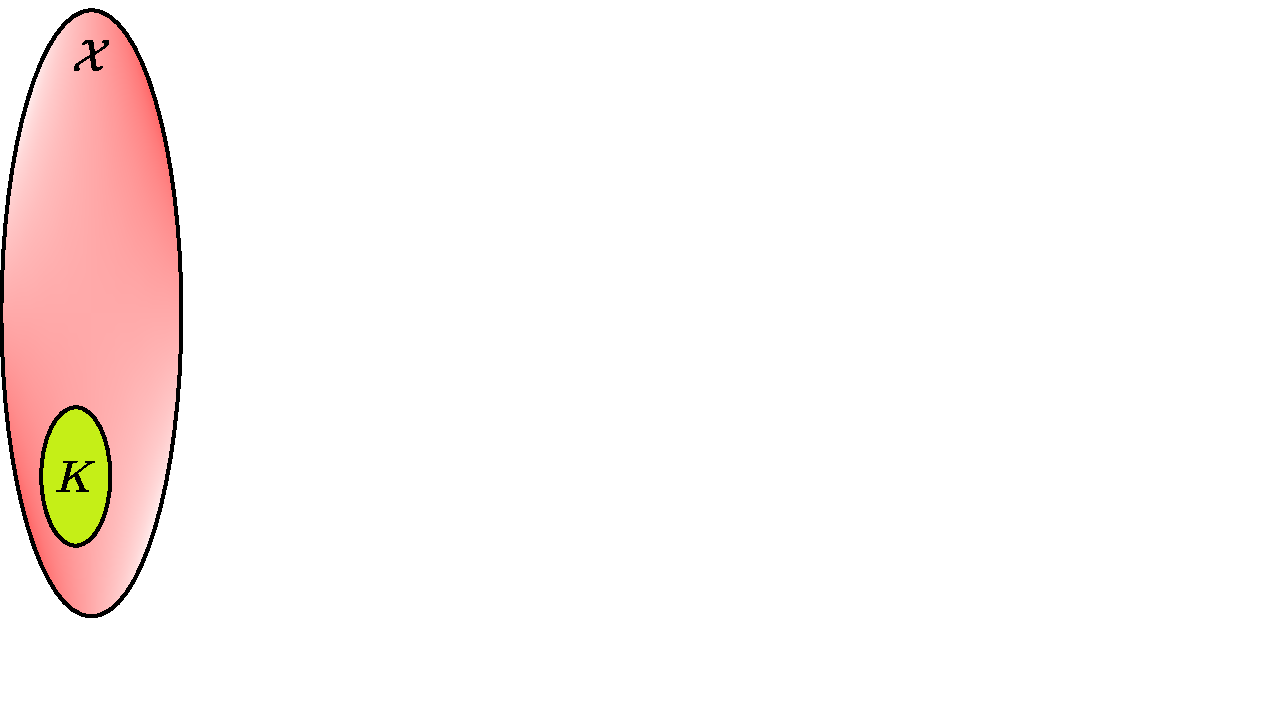
\includegraphics[width=0.9\textwidth, trim=0 0 0 0, clip]{./figures/KP1.pdf}}
      \only<2>{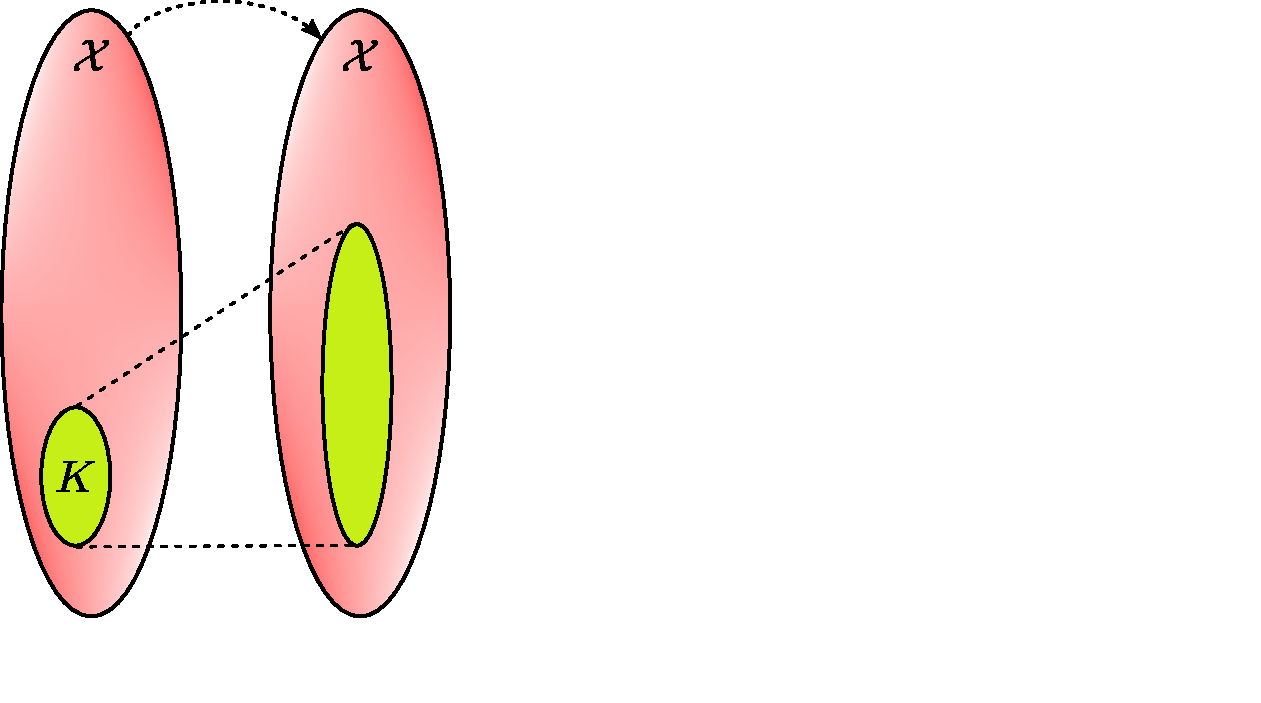
\includegraphics[width=0.9\textwidth, trim=0 0 0 0, clip]{./figures/KP2.pdf}}
      \only<3>{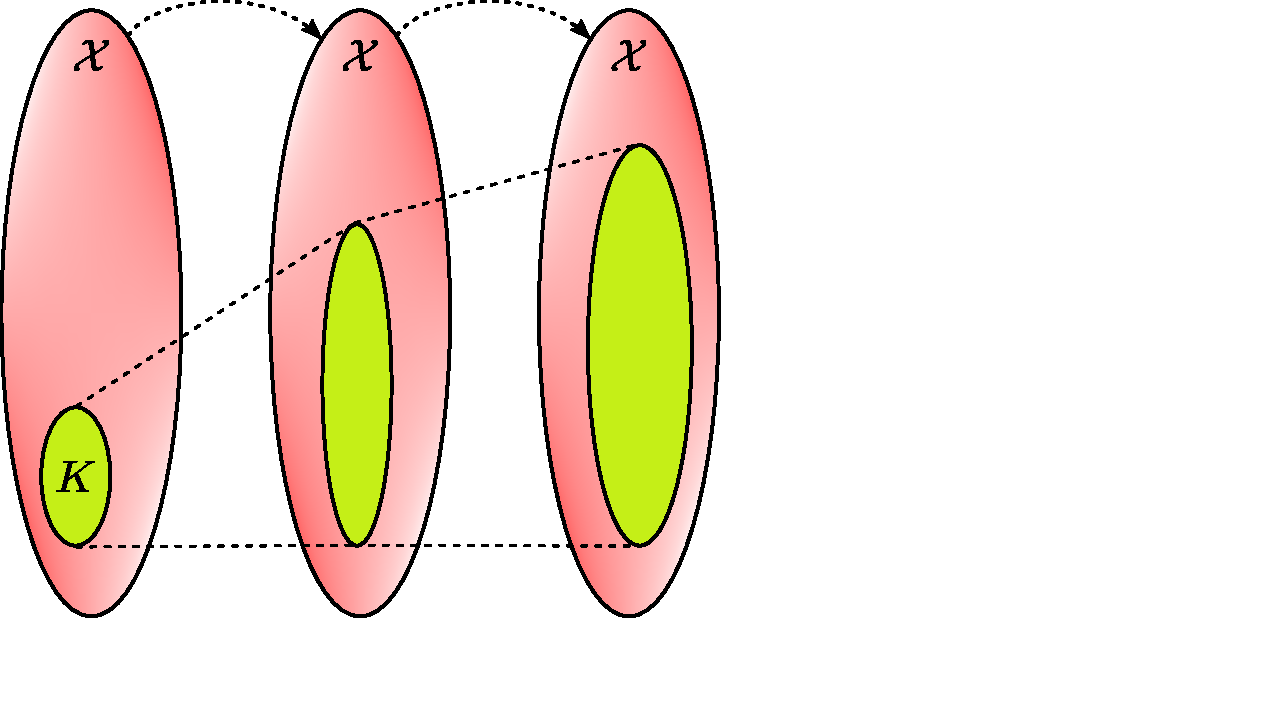
\includegraphics[width=0.9\textwidth, trim=0 0 0 0, clip]{./figures/KP3.pdf}}
      \only<4>{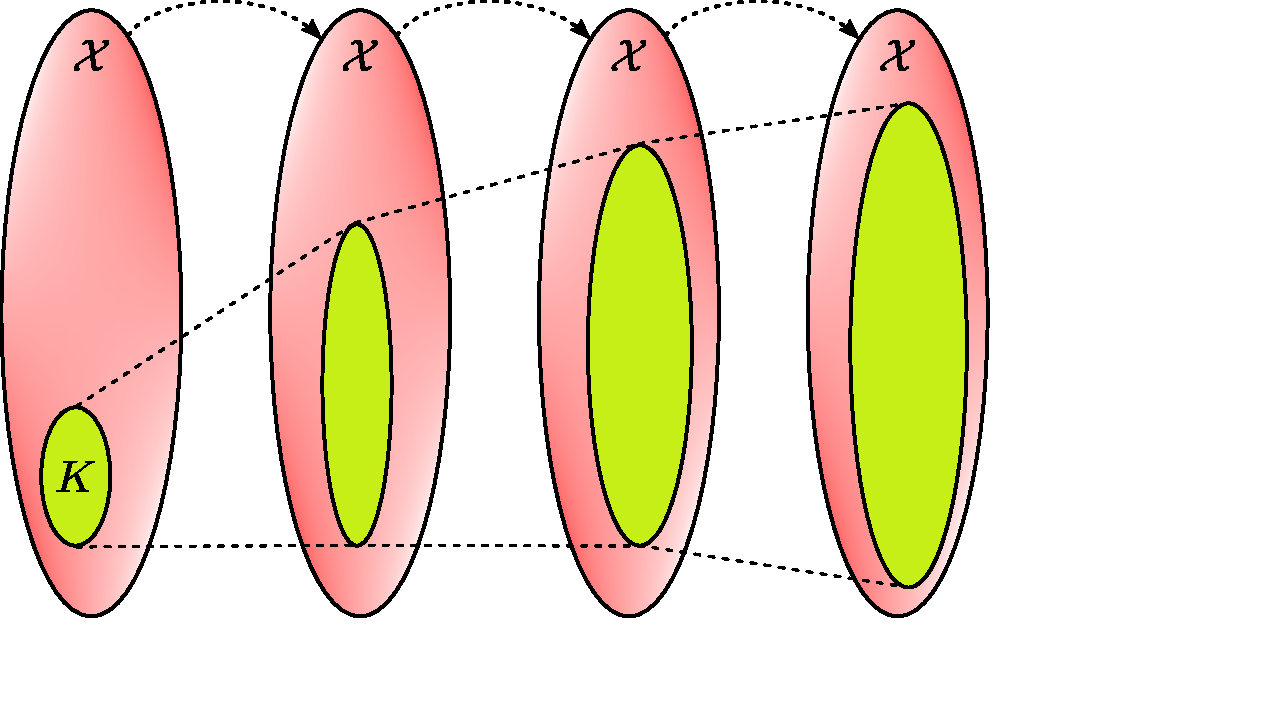
\includegraphics[width=0.9\textwidth, trim=0 0 0 0, clip]{./figures/KP4.pdf}}
      \only<5>{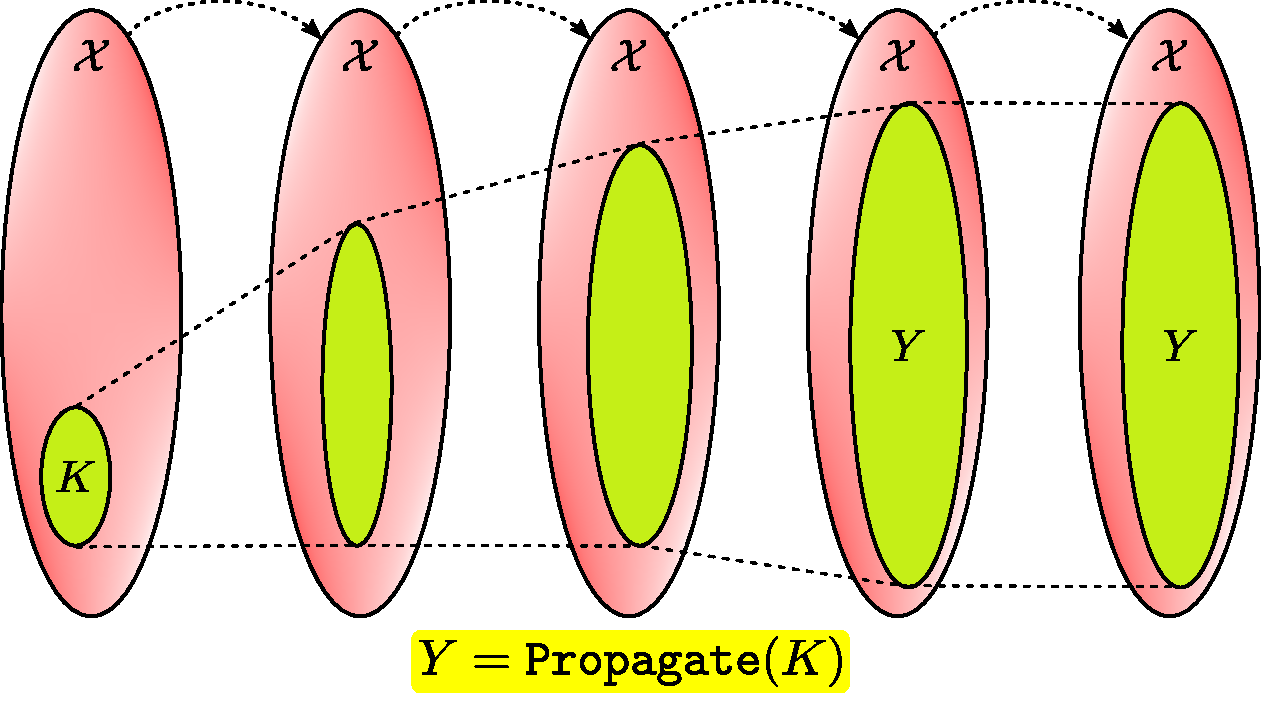
\includegraphics[width=0.9\textwidth, trim=0 0 0 0, clip]{./figures/KP5.pdf}}
      \only<6>{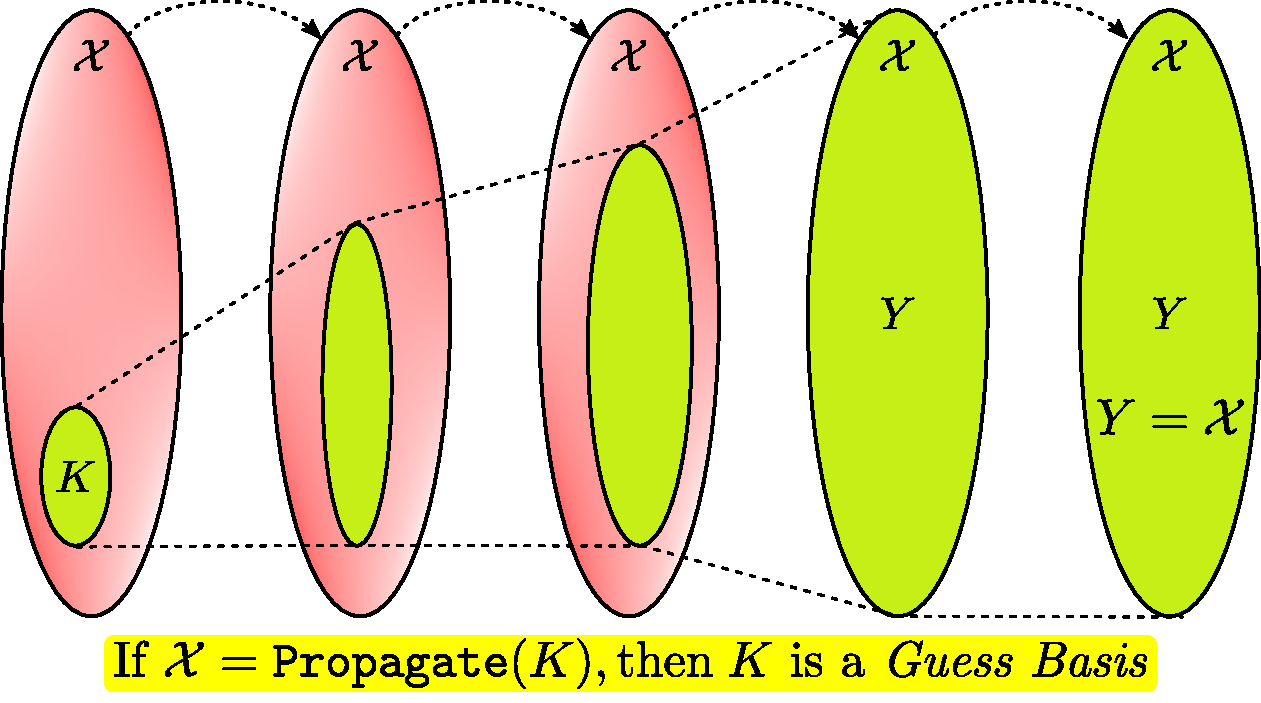
\includegraphics[width=0.9\textwidth, trim=0 0 0 0, clip]{./figures/KP6.pdf}}
      \end{overlayarea}
    \end{figure}
  \end{columns}
\end{frame}

%%%%%%%%%%%%%%%%%%%%%%%%%%%%%%%%%%%%%%%%%%%%%%%%%%%%%%%%%%%%%%%%%%%%%%%%
\begin{frame}{Naive Approach for GD}
  Given a system of relations \((\mathcal{X}, \mathcal{R})\), where $|\mathcal{X}| = n$, 
  is there any guess basis of size \(\leq m\)?
  
  \onslide<2->{%
  \begin{block}{Brute-force}
  \footnotesize
  \begin{itemize}
  \item For \(k = 1 \rightarrow m\)
  \begin{itemize}
  \item For each subset \(K \subseteq \mathcal{X}\), where \(|K| = k\):
  \begin{itemize}
  \item If \(\texttt{Propagate(K)} = \mathcal{X}\) then return \(K\)
  \end{itemize}
  \end{itemize}
  \end{itemize}
  \end{block}
  }
  \onslide<3>{
  \begin{itemize}
  \item Time complexity \(\approx \sum_{k = 1}^{m}\binom{n}{k}\)\\
  \item Exponential with respect to both $n$ and $m$
  \end{itemize}
  }
\end{frame}


%%%%%%%%%%%%%%%%%%%%%%%%%%%%%%%%%%%%%%%%%%%%%%%%%%%%%%%%%%%%%%%%%%%%%%%%
\subsection{Converting GD to a CP Problem}
% \sectionheader[\huge\color{tug}\faBook]{Converting GD to a CP Problem}
%%%%%%%%%%%%%%%%%%%%%%%%%%%%%%%%%%%%%%%%%%%%%%%%%%%%%%%%%%%%%%%%%%%%%%%%
\begin{frame}{CP-Based Approach to Solve GD Problem}
\begin{enumerate}
\small
\item Convert the system of equations to a system of relations
\begin{itemize}
  \item We can apply a preprocessing step here (Gaussian elimination)
\end{itemize}
\item Convert the problem of finding a minimal guess basis to a CP problem
\item Employ the state-of-the-art CP solvers to solve the problem
\end{enumerate}
\end{frame}

%%%%%%%%%%%%%%%%%%%%%%%%%%%%%%%%%%%%%%%%%%%%%%%%%%%%%%%%%%%%%%%%%%%%%%%%
\begin{frame}{Convert GD to a CP Problem}
\vspace{-0.5cm}
\begin{columns}
\column{0.6\textwidth}
\begin{align*}
&r_{0}: [~\hlbox<3>{green}{x}, \hlbox<4>{yellow}{y}, z]&\\
&r_{1}: [z, w, \hlbox<4>{yellow}{y}]&\\
&r_{2}: [w, \hlbox<3>{green}{x}, u]&\\
\end{align*}
\only<2>{
\vspace{-1.5cm}
% \begin{align*}
% &\text{Fix the number of steps in }\\
% &X = \{~x_{i}, y_{i}, z_{i}, w_{i}, u_{i}: 0 \leq i \leq 2\}\\
% &\text{Domain: all variables are binary}\\
% &\text{Constraints}: \mathcal{C} \gets \emptyset
% \end{align*}
\begin{itemize}
\footnotesize
\item Fix the number of steps in knowledge propagation
\item $X = \{~x_{i}, y_{i}, z_{i}, w_{i}, u_{i}: 0 \leq i \leq 2\}$
\item $x_{i} = 1$ iff $x$ is known after the $i$th step of knowledge propagation, otherwise $x_{i} = 0$
\item Initialize the set of constraints: $\mathcal{C} \gets \emptyset$
\end{itemize}
}
\only<3>{
\vspace{-1.5cm}
\begin{align*}
X \gets X &\cup \{~\hlbox<3>{green}{$x_{0, 0}$}, ~\hlbox<3>{green}{$x_{0, 1}$}\}&\\
\mathcal{C} \gets \mathcal{C} \cup &\{~\hlbox<3>{green}{$x_{0, 0}$} = y_{0} \wedge z_{0}\}&\\
\mathcal{C} \gets \mathcal{C} \cup &\{~\hlbox<3>{green}{$x_{0, 1}$} = w_{0} \wedge u_{0}\}&\\
\mathcal{C} \gets \mathcal{C} \cup &\{x_{1} = \hlbox<3>{green}{$x_{0, 0}$} \vee \hlbox<3>{green}{$x_{0, 1}$}\}&
\end{align*}
}
\only<4>{
\vspace{-1.5cm}
\begin{align*}
X \gets X &\cup \{~\hlbox<4>{yellow}{$y_{0, 0}$}, ~\hlbox<4>{yellow}{$y_{0, 1}$}\}&\\
\mathcal{C} \gets \mathcal{C} \cup &\{~\hlbox<4>{yellow}{$y_{0, 0}$} = x_{0} \wedge z_{0}\}&\\
\mathcal{C} \gets \mathcal{C} \cup &\{~\hlbox<4>{yellow}{$y_{0, 1}$} = z_{0} \wedge w_{0}\}&\\
\mathcal{C} \gets \mathcal{C} \cup &\{~\hlbox<4>{yellow}{$y_{1}$} =  \hlbox<4>{yellow}{$y_{0, 0}$} \vee \hlbox<4>{yellow}{$y_{0, 1}$}\}&
\end{align*}
}
\only<5>{
\vspace{-0.5cm}
\begin{itemize}
  \item Do it for all variables and in each step
  \item All variables should be known at the last step:
  \begin{equation*}
    \mathcal{C} \gets \mathcal{C} \cup \{x_{2} \wedge y_{2} \wedge z_{2} \wedge w_{2} \wedge u_{2} = 1\}
    \end{equation*}
\end{itemize}
}
\only<6->{
\begin{align*}
\min~&x_{0} + y_{0} + z_{0} + w_{0} + u_{0}\\
s.t.& ~\text{all constraints in} ~ \mathcal{C} ~ \text{are satisfied}
\end{align*}
}
\column{0.4\textwidth}
\only<2-6>{
\begin{figure}
\begin{tikzpicture}
\pgfmathsetmacro{\hd}{2};
\pgfmathsetmacro{\vd}{0.7};
\node[ellipse,draw] (s1) at (0, 0) {$x_{\onslide<2->{\color{tugred}{0}}}, ~ y_{\onslide<2->{\color{tugred}{0}}},  ~ z_{\onslide<2->{\color{tugred}{0}}}, ~ w_{\onslide<2->{\color{tugred}{0}}}, ~ u_{\onslide<2->{\color{tugred}{0}}}$};
\onslide<2->{
\node[ellipse,draw] (s2) at ($(s1) + (0, -2*\vd)$) {$x_{\onslide<2->{\color{tugred}{1}}}, ~ y_{\onslide<2->{\color{tugred}{1}}}, ~ z_{\onslide<2->{\color{tugred}{1}}}, ~ w_{\onslide<2->{\color{tugred}{1}}}, ~ u_{\onslide<2->{\color{tugred}{1}}}$};
\draw[>=latex, ->, rounded corners=20pt] (s1.0) -- ($0.5*(s1.0) + 0.5*(s2.0) + (0.5, 0)$) -- (s2.0);
}
\only<2->{
\node[ellipse,draw] (s3) at ($(s1) + (0, -4*\vd)$) {$x_{\color{tugred}{2}}, ~ y_{\color{tugred}{2}}, ~ z_{\color{tugred}{2}}, ~ w_{\color{tugred}{2}}, ~ u_{\color{tugred}{2}}$};
\draw[>=latex, ->, rounded corners=20pt] (s2.0) -- ($0.5*(s2.0) + 0.5*(s3.0) + (0.5, 0)$) -- (s3.0);
\node[ellipse] (s4) at ($(s1) + (0, -6*\vd)$) {$\textcolor{white}{x_{2}, ~ y_{2},~ z_{2}, ~ w_{2}, ~ u_{2}}$};
% \draw[>=latex, dashed, ->, rounded corners=20pt] (s3.0) -- ($0.5*(s3.0) + 0.5*(s4.0) + (0.5, 0)$) -- (s4.0);
}
% \only<7->{
% \node[ellipse,draw] (s3) at ($(s1) + (0, -4*\vd)$) {$x_{\color{tugred}{2}}, ~ y_{\color{tugred}{2}}, ~ z_{\color{tugred}{2}}, ~ w_{\color{tugred}{2}}, ~ u_{\color{tugred}{2}}$};
% \draw[>=latex, ->, rounded corners=20pt] (s2.0) -- ($0.5*(s2.0) + 0.5*(s3.0) + (0.5, 0)$) -- (s3.0);
% }
% \draw[->] (n1) -- (n2);
% \draw[->] (d1) -- (n1);
% \draw[->] (d2) -- (n2);
\end{tikzpicture}
\end{figure}
}
\only<7>{
\begin{figure}
\centering
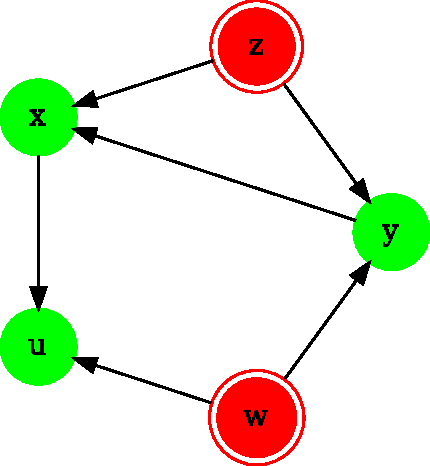
\includegraphics[width=0.57\textwidth]{./figures/dg_example.pdf}
\end{figure}
}
\end{columns}
\end{frame}

%%%%%%%%%%%%%%%%%%%%%%%%%%%%%%%%%%%%%%%%%%%%%%%%%%%%%%%%%%%%%%%%%%%%%%%%
\begin{frame}{Autoguess}
  \vspace{-0.47cm}
  \begin{figure}
  \centering
  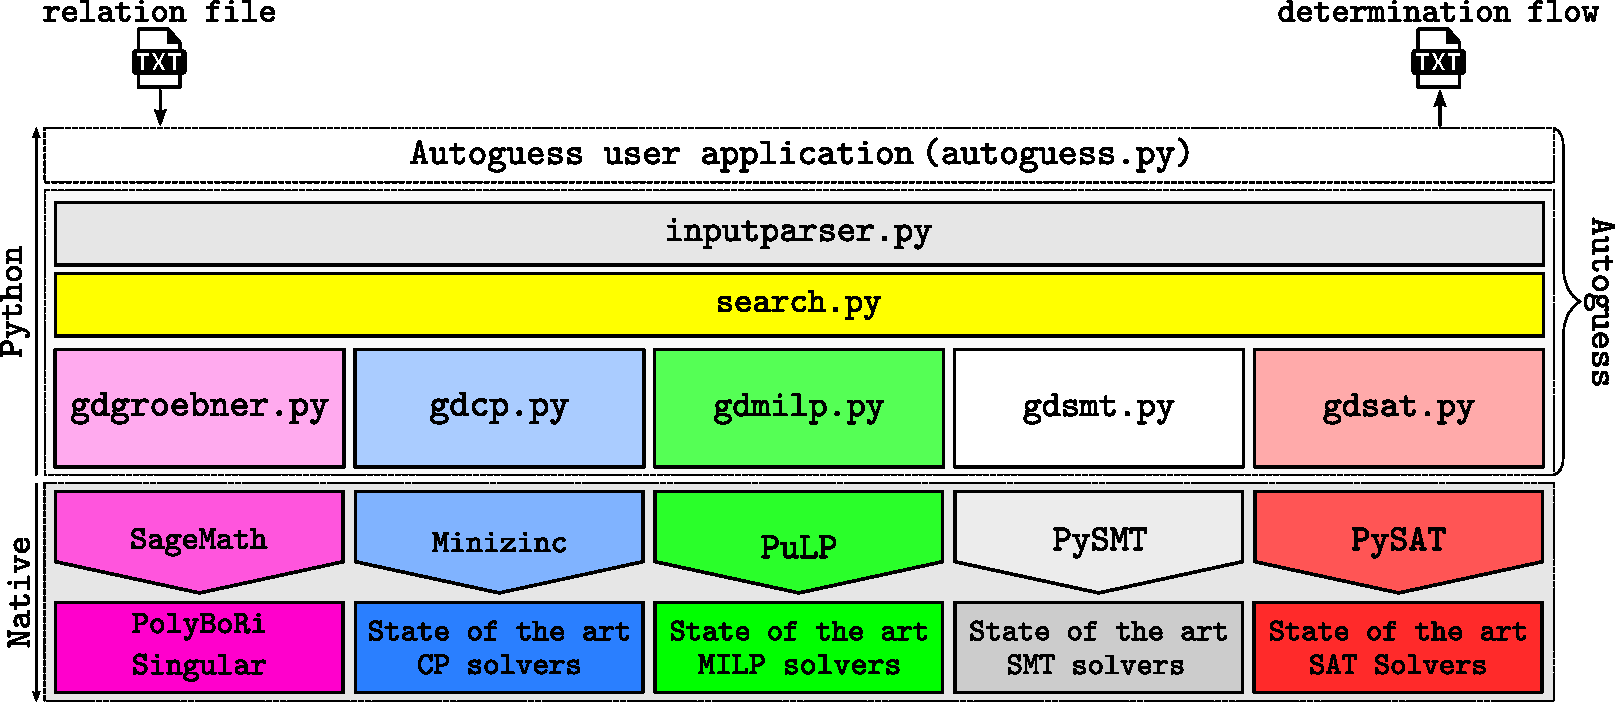
\includegraphics[width=0.9\textwidth]{./figures/autoguess_design.pdf}
  \end{figure}
  \begin{center}
    \faGithub: \url{https://github.com/hadipourh/autoguess}
  \end{center}
\end{frame}

%%%%%%%%%%%%%%%%%%%%%%%%%%%%%%%%%%%%%%%%%%%%%%%%%%%%%%%%%%%%%%%%%%%%%%%%
\begin{frame}{Autoguess - Simple User Interface}
  \vspace{-0.5cm}
  \begin{columns}
  \column{0.5\textwidth}
  \only<1>{
  {\footnotesize
  \begin{align*}
  \quad \left \{ \begin{array}{lr}
  F(u + v) \oplus G(x) \oplus y \oplus (z \lll 7) &= c_{1}\\
  G(u \oplus w) + (y \lll 3) + z &= c_{2}\\
  F(w \oplus x) + y \oplus z &= c_{3}\\
  F(u) \oplus G(w + z) &= c_{4}\\
  \left(F(u) \times G(w\lll 7)\right) + H(z\oplus v) &= c_{5}\\
  \end{array} \right.
  \end{align*}
  }
  }
  \only<2->{
  {\footnotesize
  Input file (\texttt{relations.txt}):\\
  }
  \begin{center}
  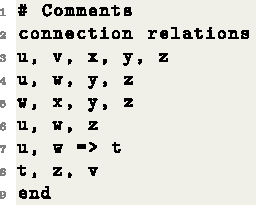
\includegraphics[scale=1]{figures/autoguess_inputfile.pdf}
  \end{center}
  }
  \vspace{0.7cm}
  \only<2->{
  {\footnotesize
  Run Autoguess:\\
  }
  {\footnotesize
  \colorbox{darkgray}{\textcolor{white}{\texttt{python3 autoguess.py -i relations.txt --maxsteps 5 --solver cp}}}
  }
  }
  \column{0.5\textwidth}
  \only<3>{
  {\footnotesize
  Output:\\
  }
  \centering
  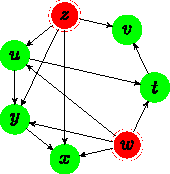
\includegraphics[width=0.55\textwidth]{figures/autoguess_usage.pdf}
  }
  \end{columns}
\end{frame}

%%%%%%%%%%%%%%%%%%%%%%%%%%%%%%%%%%%%%%%%%%%%%%%%%%%%%%%%%%%%%%%%%%%%%%%%
\subsection{Some Applications of Autoguess}
% \sectionheader[\huge\color{tug}\faBook]{Some Applications of Autoguess}
%%%%%%%%%%%%%%%%%%%%%%%%%%%%%%%%%%%%%%%%%%%%%%%%%%%%%%%%%%%%%%%%%%%%%%%%
\begin{frame}{GD Attack on 1 to 3 Rounds of \cipher{AES}}
\vspace{-0.4cm}
\begin{columns}
\column{0.5\textwidth}
  \begin{center}
    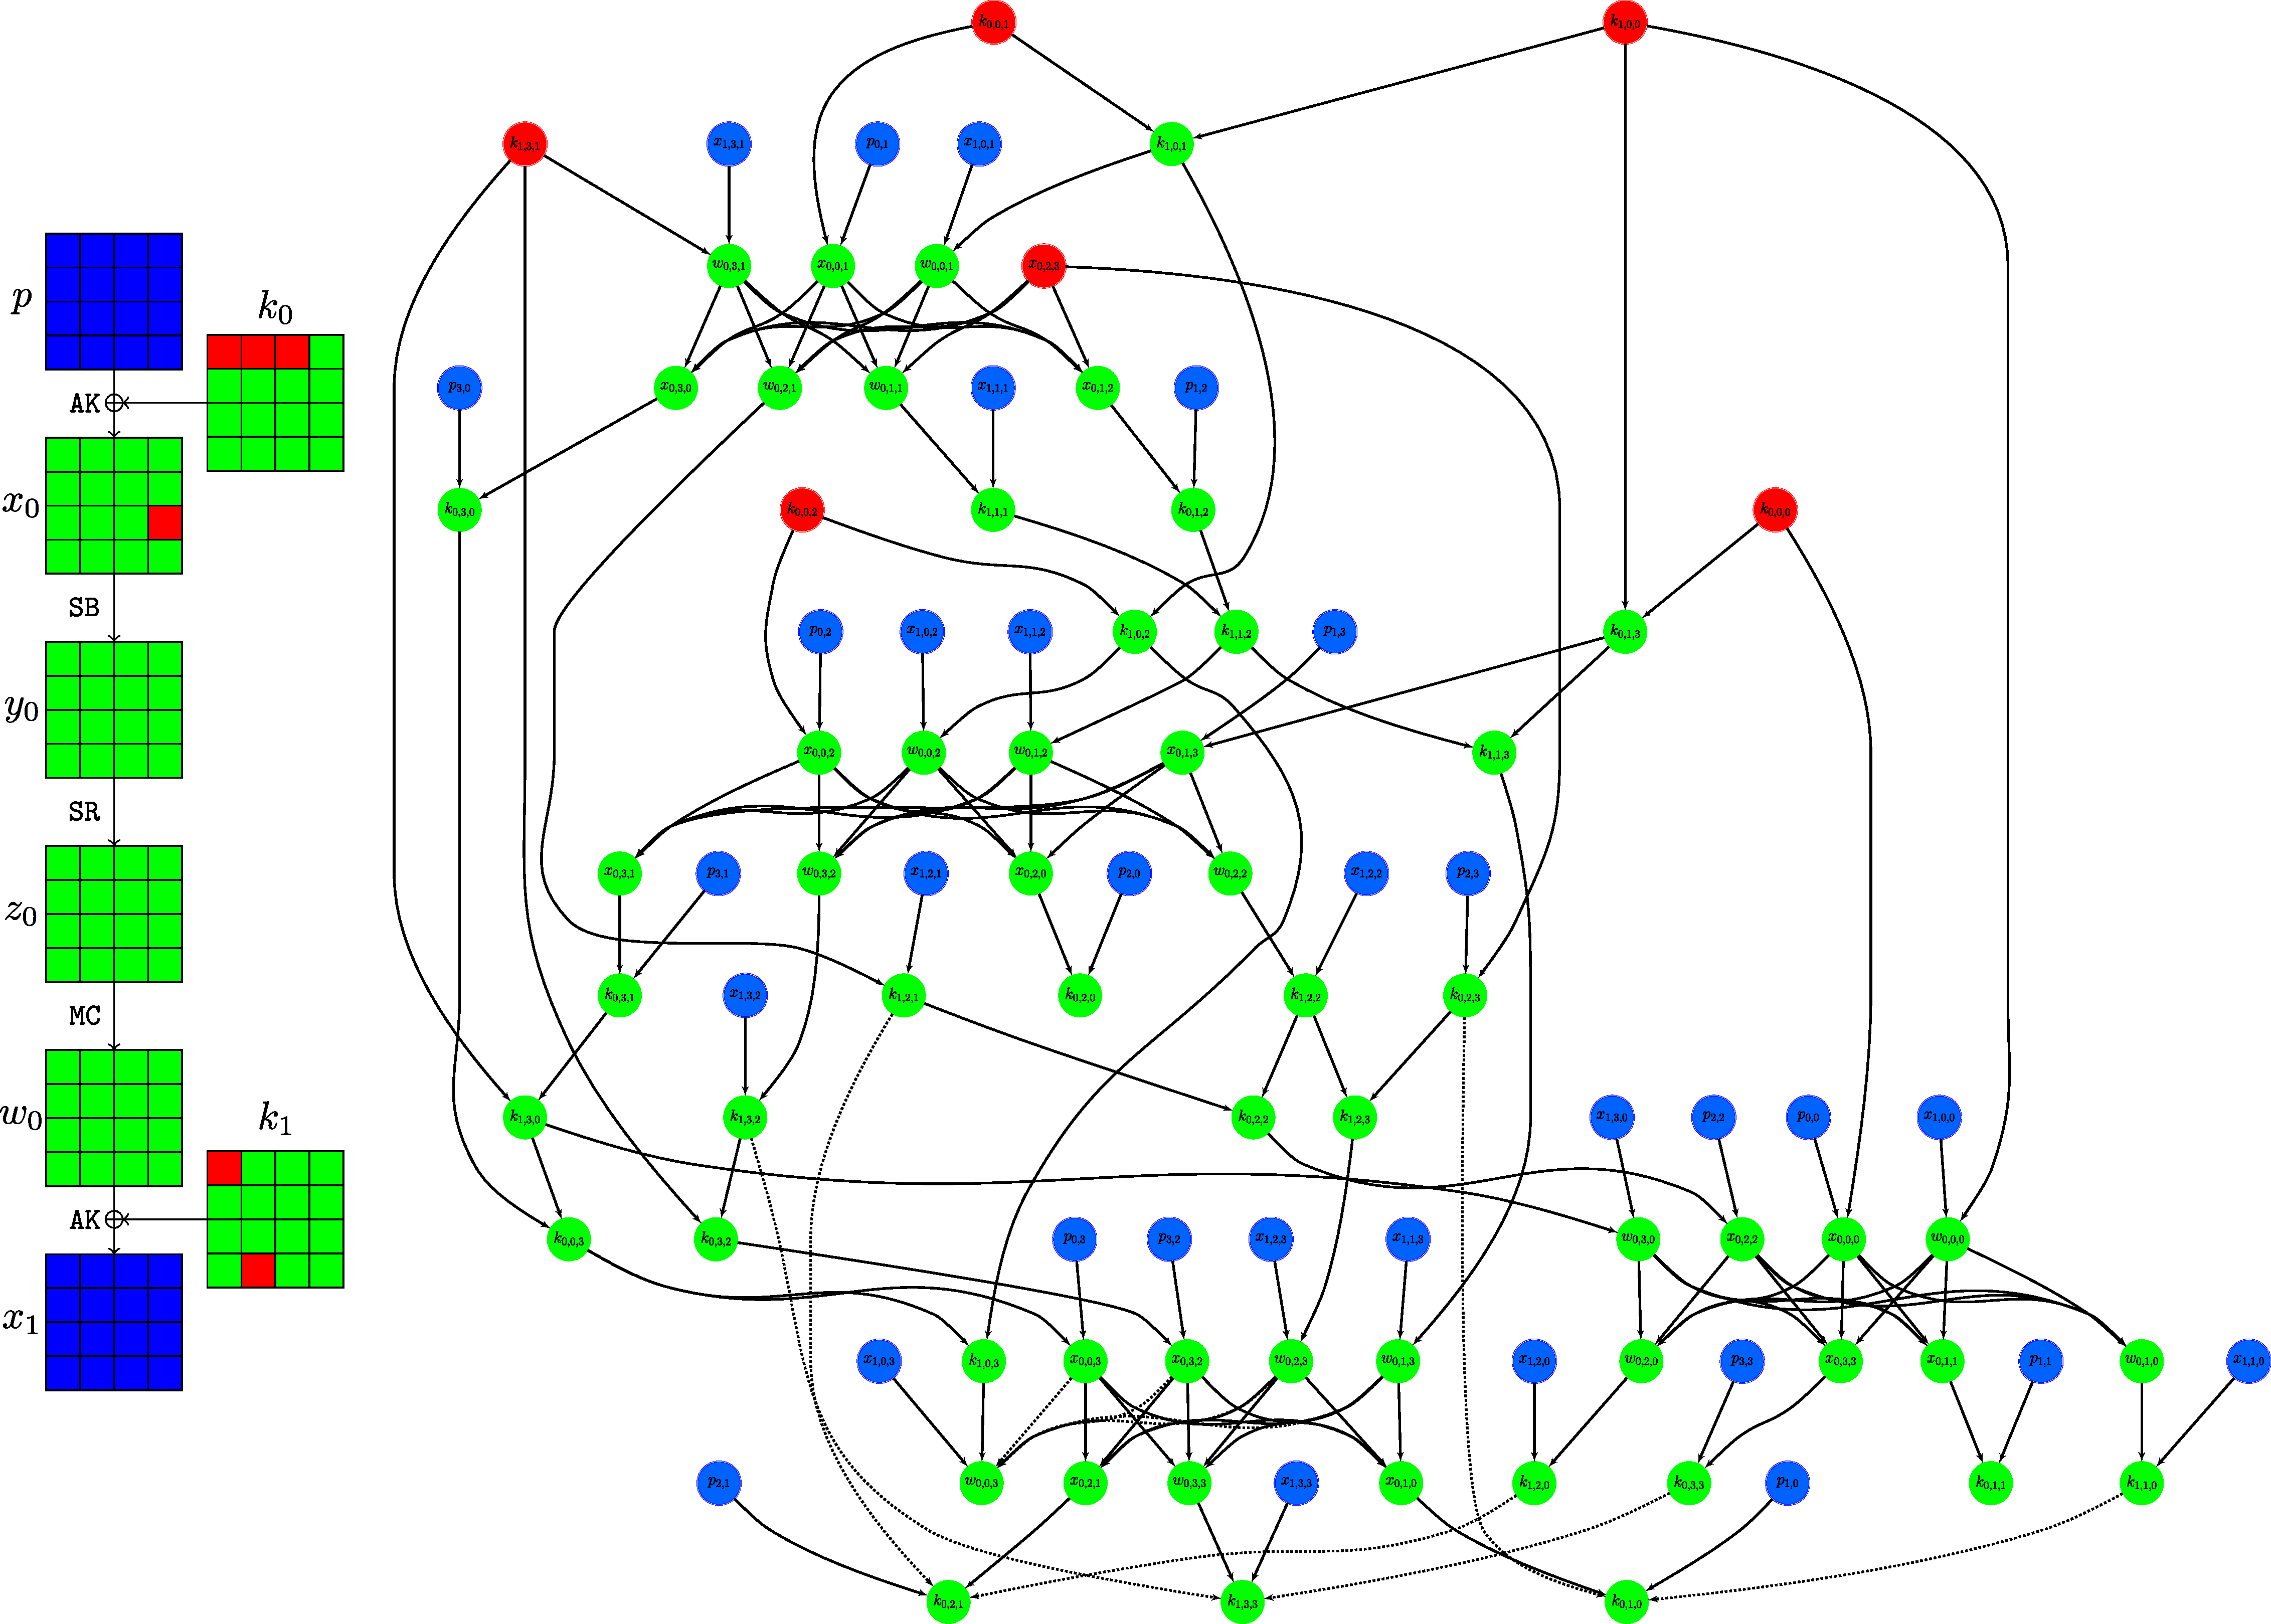
\includegraphics[width=\textwidth]{./figures/aes_1_round_gd_dg.pdf}
  \end{center}
  \vspace{-0.2cm}
  \scriptsize
  \centering
  Found in \colorbox{gold}{0.02 seconds} on a standard laptop
\column{0.5\textwidth}
  \begin{center}
    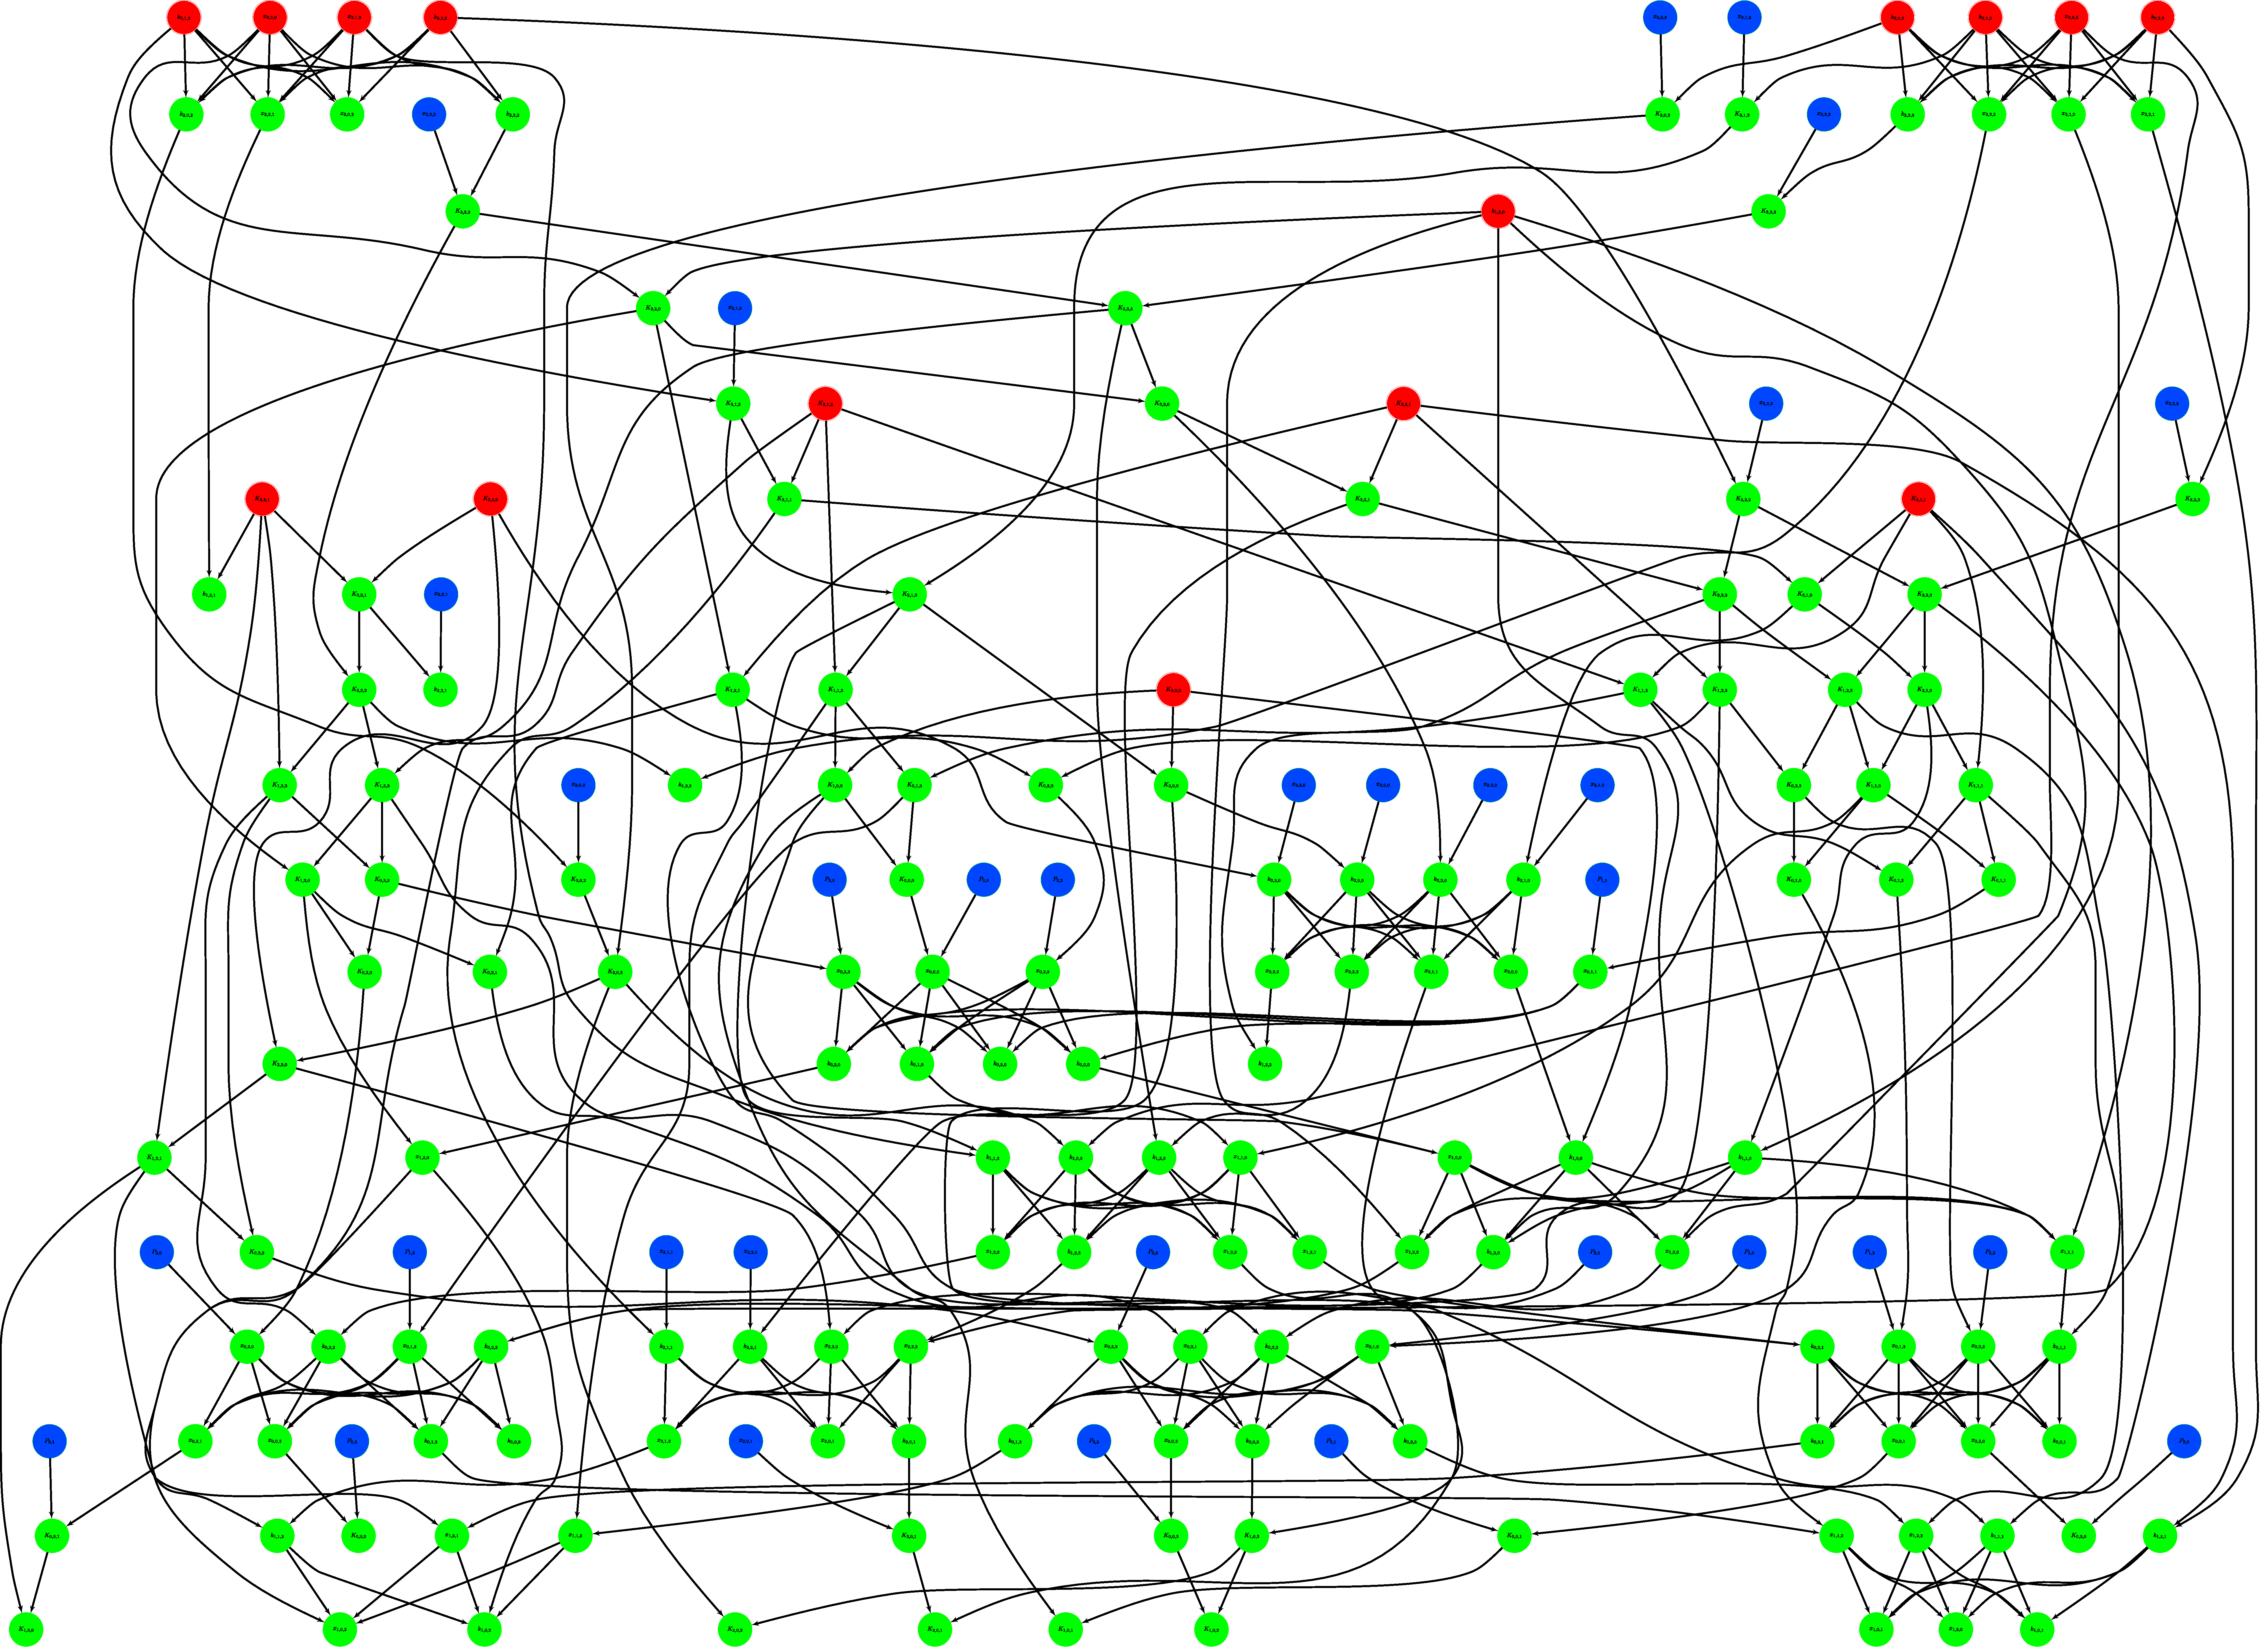
\includegraphics[width=\textwidth]{figures/aes_3_rounds_gd_dg.pdf}
  \end{center}
  \vspace{-0.2cm}
  \scriptsize
  \centering
  Found in \colorbox{gold}{34.51 seconds} on a standard laptop
\end{columns}
\end{frame}

%%%%%%%%%%%%%%%%%%%%%%%%%%%%%%%%%%%%%%%%%%%%%%%%%%%%%%%%%%%%%%%%%%%%%%%%
\begin{frame}{GD Attack on KCipher-2}
\vspace{-0.6cm}
\begin{columns}
\column{0.5\textwidth}
  \begin{center}
  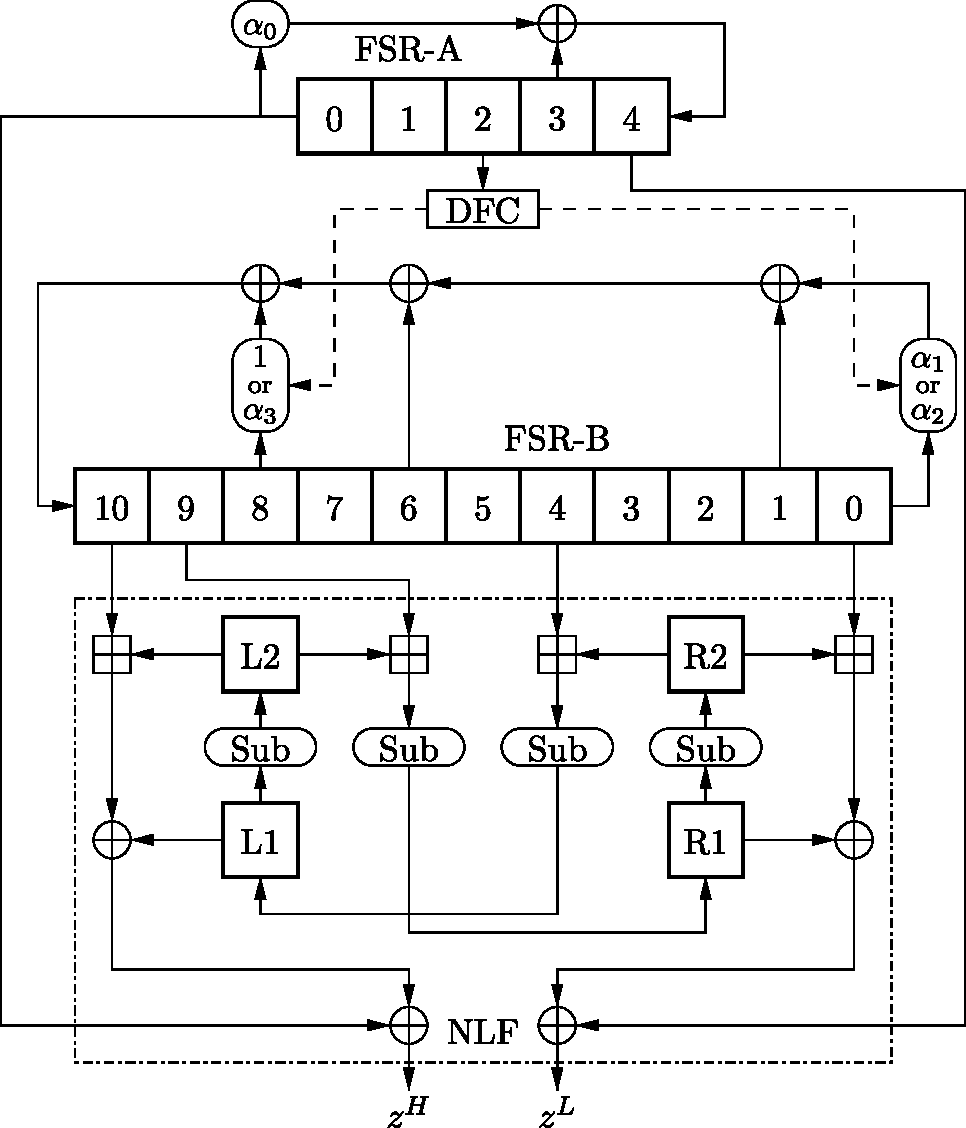
\includegraphics[scale=0.30, clip]{figures/kcipher2.pdf}\\
  \vspace{-0.1cm}
  \href{https://www.iso.org/standard/54532.html}{ISO/IEC 18033-4}
  \end{center}
\column{0.5\textwidth}
  \begin{center}
  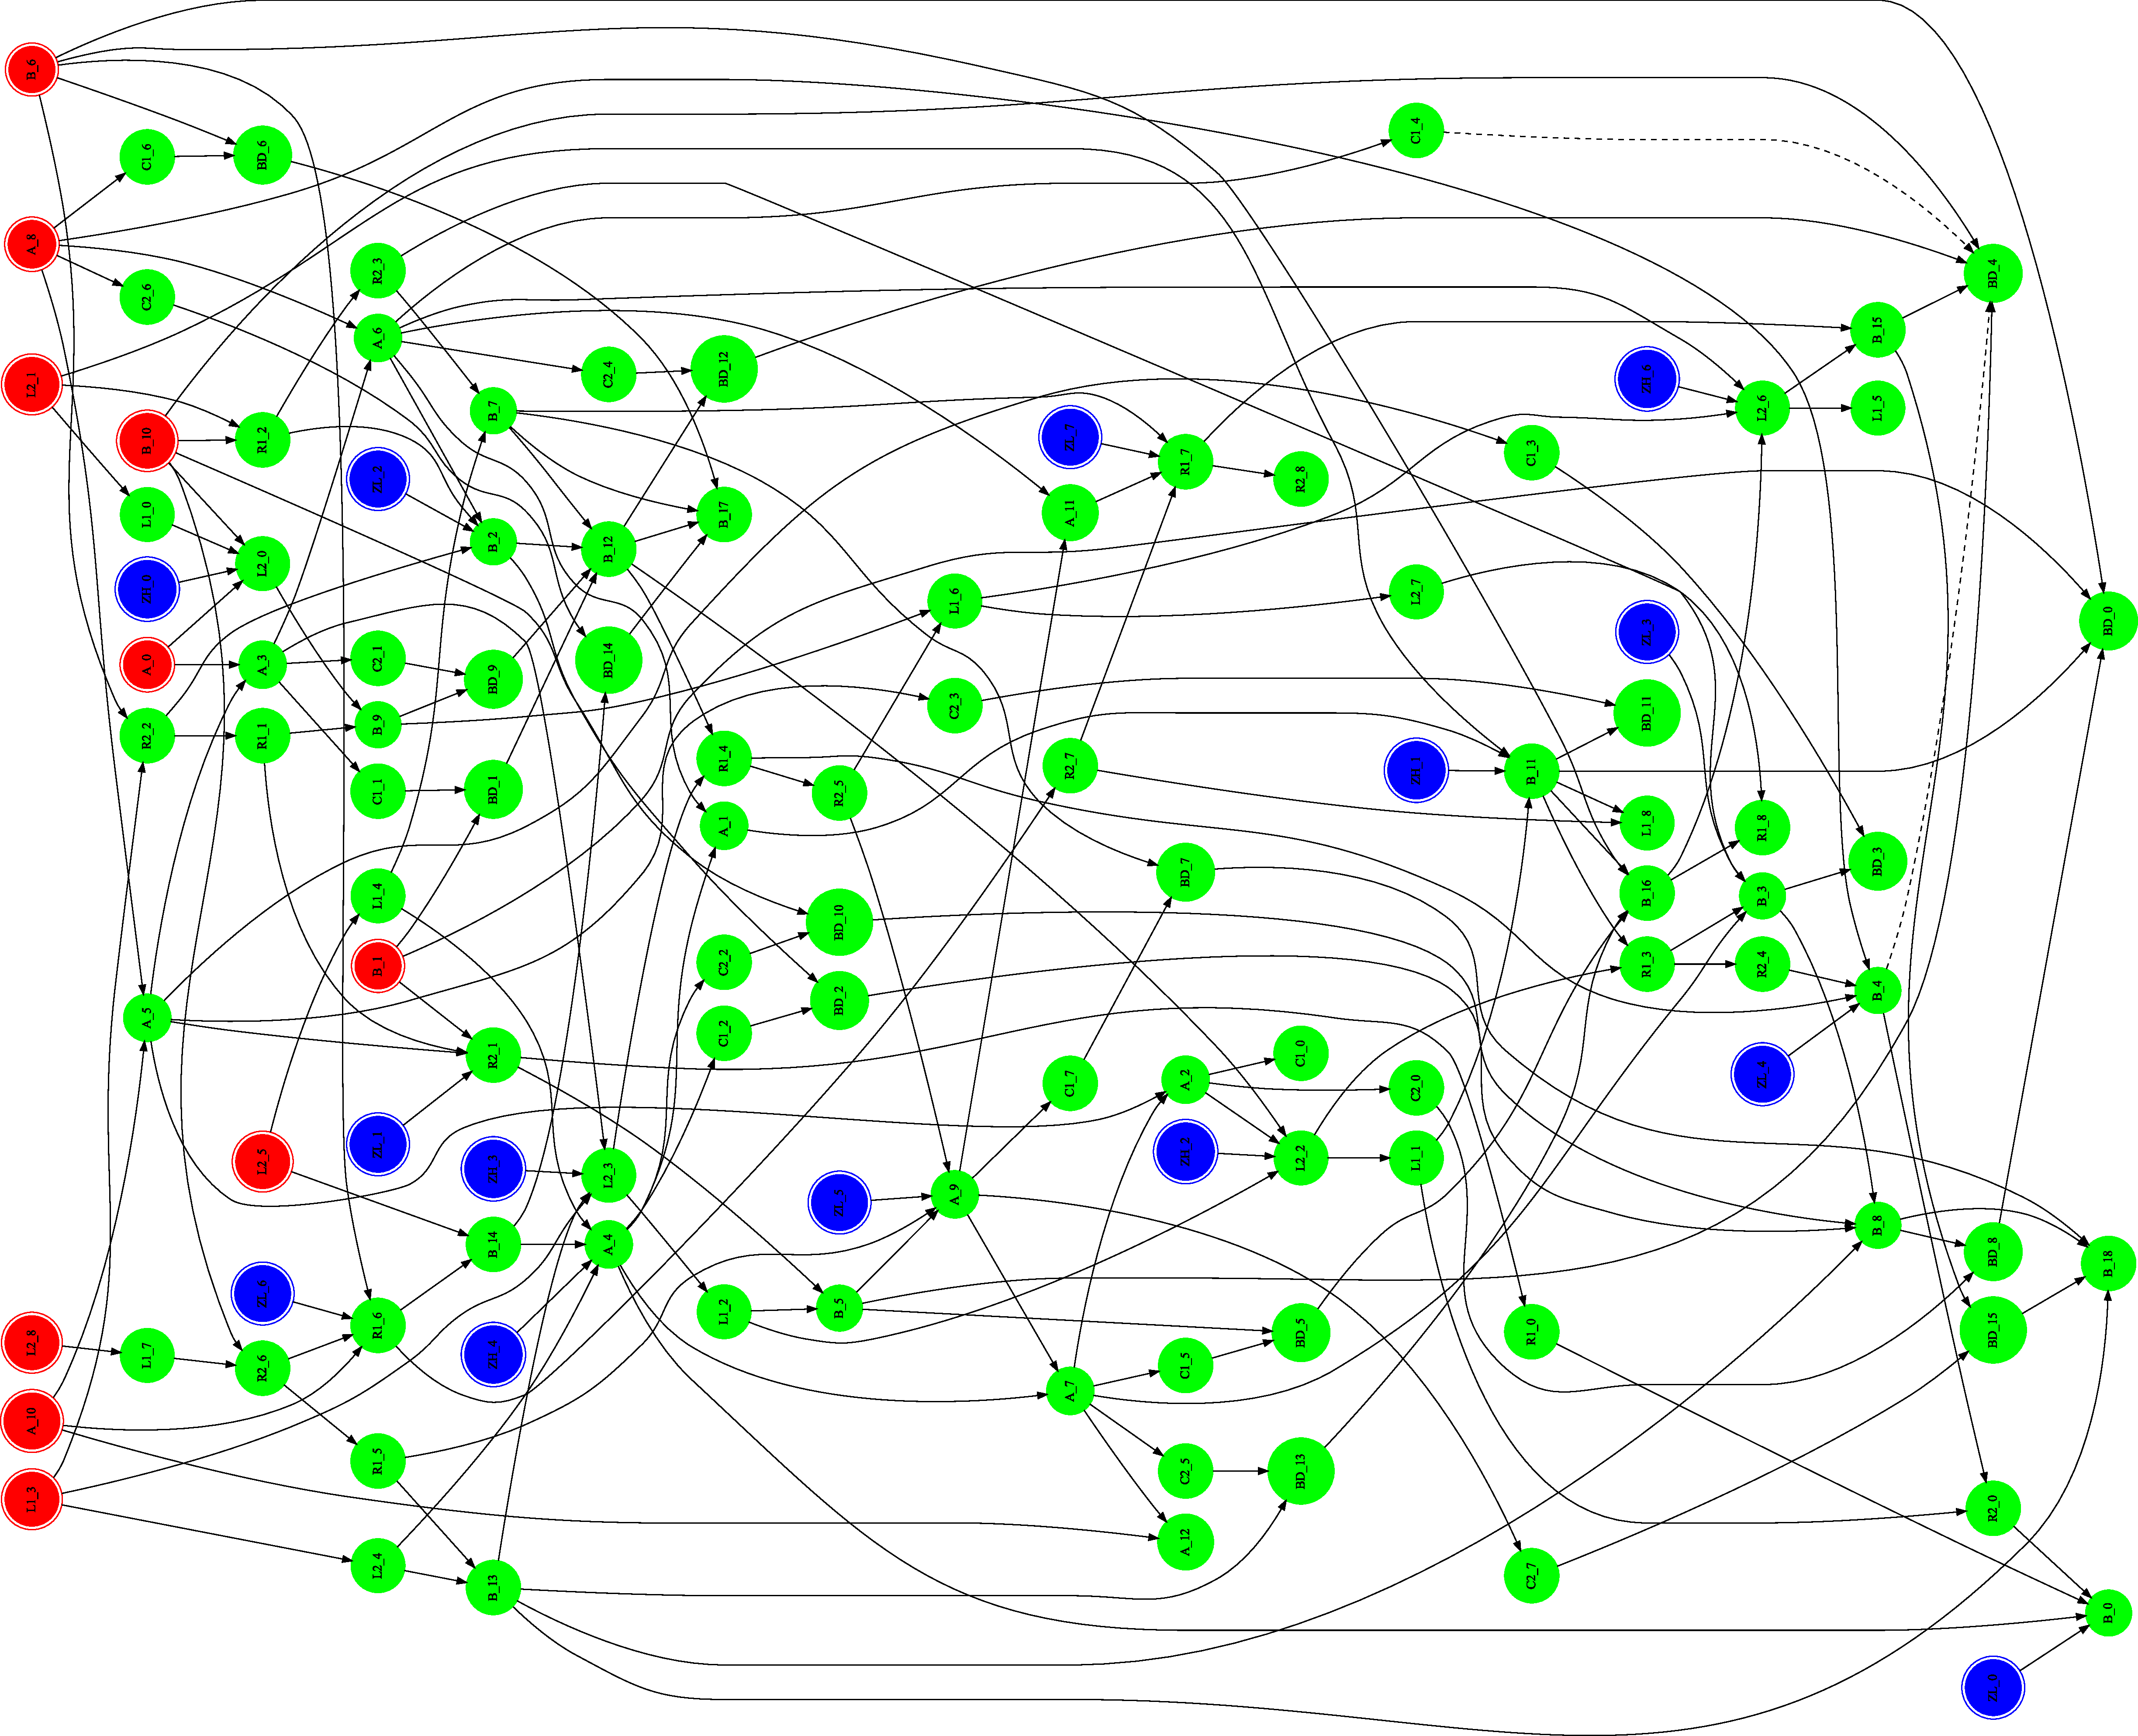
\includegraphics[width=0.75\textwidth, clip]{figures/kcipher2_8clks_10g_19s_gd_dg.pdf}\\
  \vspace{-0.1cm}
  Found in \colorbox{gold}{7 seconds} on a standard laptop
  \end{center}
\end{columns}
\end{frame}

%%%%%%%%%%%%%%%%%%%%%%%%%%%%%%%%%%%%%%%%%%%%%%%%%%%%%%%%%%%%%%%%%%%%%%%%
%%%%%%%%%%%%%%%%%%%%%%%%%%%%%%%%%%%%%%%%%%%%%%%%%%%%%%%%%%%%%%%%%%%%%%%%
\section{Conclusion and Our Other Contributions}
\sectionheader[\huge\color{tug}\faHourglassEnd]{Conclusion and Our Other Contributions}

%%%%%%%%%%%%%%%%%%%%%%%%%%%%%%%%%%%%%%%%%%%%%%%%%%%%%%%%%%%%%%%%%%%%%%%%
\begin{frame}{Our Contributions -- I}
\begin{itemize}
  \footnotesize
  \item[\faCheckCircle] \fullcite{eurocrypt_HadipourSE23}
  \item[\faCheckCircle] \fullcite{tosc_HadipourNE22}
  \item[\faCheckCircle] \fullcite{tosc_HadipourE22}
\end{itemize}
\end{frame}

%%%%%%%%%%%%%%%%%%%%%%%%%%%%%%%%%%%%%%%%%%%%%%%%%%%%%%%%%%%%%%%%%%%%%%%%
\begin{frame}{Our Contributions -- II}
\begin{itemize}
  \footnotesize
  \item[\faCheckCircle] \fullcite{acns_HadipourE22}
  \item[\faCheckCircle] \fullcite{eprint_HadipourGSE23}
  \item[\faCheckCircle] \fullcite{eprint_HadipourT23}
\end{itemize}
\end{frame}

%%%%%%%%%%%%%%%%%%%%%%%%%%%%%%%%%%%%%%%%%%%%%%%%%%%%%%%%%%%%%%%%%%%%%%%%
\begin{frame}{Future Works}
\vspace{-0.5cm}
\begin{itemize}
\item Future works
\begin{itemize}
\small
\item[\faRoad] Improving the accuracy and performance of the existing automated methods
\item[\faRoad] Many cryptanalytic methods are not automated yet
\item[\faRoad] New cryptanalytic methods require new automated tools
\end{itemize} 
\end{itemize}
\begin{center}
\vspace{0.10cm}

{\large Thanks for your attention!}

\vspace{0.3cm}
\faGithub: \url{https://github.com/hadipourh/talks}\\
% \vspace{0.1cm}
% \faArchive: \url{https://ia.cr/2022/1147}
\end{center}
\end{frame}

%%%%%%%%%%%%%%%%%%%%%%%%%%%%%%%%%%%%%%%%%%%%%%%%%%%%%%%%%%%%%%%%%%%%%%%%%%%%

\begin{frame}[allowframebreaks]{Bibliography}
  \printbibliography
\end{frame}

%%%%%%%%%%%%%%%%%%%%%%%%%%%%%%%%%%%%%%%%%%%%%%%%%%%%%%%%%%%%%%%%%%%%%%%%%%%%


%%%%%%%%%%%%%%%%%%%%%%%%%%%%%%%%%%%%%%%%%%%%%%%%%%%%%%%%%%%%%%%%%%%%%%%%%%%%
% Bakcup slides
\tikzset{stateopts/.style={scale=.50,thick}, cellopts/.style={font=\scriptsize},
         raster/.style={thin,gray!50}}
%%%%%%%%%%%%%%%%%%%%%%%%%%%%%%%%%%%%%%%%%%%%%%%%%%%%%%%%%%%%%%%%%%%%%%%%
\begin{frame}{\cipher{AES} \cite{daemen1999aes}}
\begin{itemize}
  \item Block size $n=128$ bits, Key size \emph{$k\in \{128, 192, 256\}$} bits
  \item 3 Block ciphers named after their key size: \cipher{\color{main}AES-128}, \cipher{\color{main!70}AES-192}, \cipher{\color{main!40}AES-256}
    \pause
  \item The 16-byte input block
    $M = s_{00} \Vert s_{10} \Vert s_{20} \Vert s_{30} \Vert s_{01} \Vert \dots \Vert s_{33}$
    is written as a $4 \times 4$ matrix of bytes, the \emph{$\{16, {\color{main!70}24}, {\color{main!40}32}\}$-byte} key
    \emph{$K$} % = k_{00} \Vert k_{10} \Vert \dots \Vert k_{3\{3,5,7\}}$
    as a \emph{$4 \times \{4, {\color{main!70}6}, {\color{main!40}8}\}$} matrix:
    \[{M = \tikz[baseline]{\node[state] {\State{
      \foreach \x in {0,...,3} \foreach \y in {0,...,3} \Cell{ss\x\y}{$s_{\x\y}$} 
      }};}},
      \qquad
      K = \tikz[baseline]{\node[state] {\State{
        \foreach \x in {0,...,3} { \foreach \y in {0,...,3} { \Cell{ss\x\y}{$k_{\x\y}$} } }
        \foreach \x in {0,...,3} { \foreach \y in {4,...,5} { \Cell{\y+.5,-\x-.5}{\color{main!70}$k_{\x\y}$} } }
        \foreach \x in {0,...,3} { \foreach \y in {6,...,7} { \Cell{\y+.5,-\x-.5}{\color{main!40}$k_{\x\y}$} } }
        \draw[main!70] (4,0) -- ++(2,0) -- ++(0,-4) -- ++(-2,0);
        \draw[raster]  (4,0) ++(0,-4) ++(0,1) -- +(2,0) ++(0,1) -- +(2,0) ++(0,1) -- +(2,0) ++(1,1) -- +(0,-4);
        \draw[main!40] (6,0) -- ++(2,0) -- ++(0,-4) -- ++(-2,0);
        \draw[raster]  (6,0) ++(0,-4) ++(0,1) -- +(2,0) ++(0,1) -- +(2,0) ++(0,1) -- +(2,0) ++(1,1) -- +(0,-4);
      }};}
      %\tag{for \cipher{AES-128}}
    \]
  \item The state is initialized to $M$ and updated in \emph{10 rounds} (for \cipher{\color{main}AES-128})\\
    or \textcolor{main!70}{12} rounds (\cipher{\color{main!70}AES-192})
    or \textcolor{main!40}{14} rounds (\cipher{\color{main!40}AES-256}).
    The last round is different.
\end{itemize}
\end{frame}

\newcommand{\labelAESstate}[1]{\foreach \x in {0,...,3} {
                               \foreach \y in {0,...,3} {
                                 \Cell{ss\x\y}{\scriptsize$#1_{\x\y}$}
                               }}
}
\newcommand{\tikzwrap}[2][tmp]{\tikz[baseline=(#1.base),remember picture]{\node[inner sep=0pt] (#1) {#2};}} % to point to text elements
\tikzset{stateopts/.style={scale=.45,remember picture},
  cellopts/.style={font=\scriptsize},
  statehighlight/.style={draw,fill=tugblue,minimum size=.6cm,inner sep=2pt,font=\color{white}},
}
%%%%%%%%%%%%%%%%%%%%%%%%%%%%%%%%%%%%%%%%%%%%%%%%%%%%%%%%%%%%%%%%%%%%%%%%
{\setlength{\tabcolsep}{2pt}
  \renewcommand{\arraystretch}{0.75}
\begin{frame}{\cipher{AES} Round Function -- Overview}%{{{
%\begin{frame}{}%{{{
  \vspace{-0.5cm}
  \sparen
  \sparen
  \begin{columns}
    \column{.4\textwidth}
    \begin{block}{\colbox{1} \cipher{SubBytes} (\cipher{SB})}
      \centering
      \scalebox{.9}{%
      \begin{tikzpicture}[remember picture,>=latex,xscale=0.8]
        \draw (0,0) node[state,fill=white] (X) {\State{\labelAESstate{a} }};
        \draw (ss12) node[statehighlight] (aij) {\vphantom{$b$}$a_{ij}$};
        \draw (4,0) node[state,fill=white] (Y) {\State{\labelAESstate{b} }};
        \draw (ss12) node[statehighlight] (bij) {$b_{ij}$};
  
        \draw (2,1.6) node[box,below] (S) {$\mathcal{S}$};
        \draw[tugblue,very thick,->,out=80,in=180] (aij.north) to (S.west);
        \draw[tugblue,very thick,->,out=0,in=110] (S.east) to (bij.north);
  
        \draw (X.south) ++(0,-.175) coordinate (phantom);
      \end{tikzpicture}%
      }
    \end{block}
    %\medskip

    \begin{block}{\colbox{2} \cipher{ShiftRows} (\cipher{SR})}
      \centering
      \scalebox{.9}{%
      \begin{tikzpicture}[remember picture,>=latex,xscale=0.8]
        \draw (0,0) node[state,fill=white] (X) {\State{\FillColumn[tuggreen!0]{0}
                                                       \FillColumn[tuggreen!25]{1}
                                                       \FillColumn[tuggreen!50]{2}
                                                       \FillColumn[tuggreen!75]{3}
                                                       \labelAESstate{a} }};
        \coordinate (a00) at (ss00);
        \draw (4,0) node[state,fill=white] (Y) {\State{\FillAntiDiagonal[tuggreen!0]{0}
                                                       \FillAntiDiagonal[tuggreen!25]{1}
                                                       \FillAntiDiagonal[tuggreen!50]{2}
                                                       \FillAntiDiagonal[tuggreen!75]{3}
                                                       \labelAESstate{b} }};
        \draw[tugblue,line width=3pt,->] (a00|-ss00) -- (ss00);
        \draw[tugblue,line width=3pt,->] (a00|-ss10) -- (ss13);
        \draw[tugblue,line width=3pt,->] (a00|-ss20) -- (ss22);
        \draw[tugblue,line width=3pt,->] (a00|-ss30) -- (ss31);
      \end{tikzpicture}%
      }
    \end{block}

    \column{.55\textwidth}
    \begin{block}{\colbox{3} \cipher{MixColumns} (\cipher{MC})}
      \centering
      \scalebox{.9}{%
      \begin{tikzpicture}[remember picture,>=latex,xscale=1.3]
        \draw (0,0) node[state,fill=white] (X) {\State{\labelAESstate{a}
                                                       \draw (ss12) ++(0,-.5) coordinate (col2a);}};
        \draw (ss12) node[statehighlight] (aij) {\vphantom{$b$}$a_{ij}$};
        \draw (4,0) node[state,fill=white] (Y) {\State{\labelAESstate{b}
                                                       \draw (ss12) ++(0,-.5) coordinate (col2b);}};
  
        \draw (2,1.6) node[box,below] (S) {\small$\otimes\left[\begin{array}{@{\,}c@{~}c@{~}c@{~}c@{\,}}
              \texttt{2} & \texttt{3} & \texttt{1} & \texttt{1} \\
              \texttt{1} & \texttt{2} & \texttt{3} & \texttt{1} \\
              \texttt{1} & \texttt{1} & \texttt{2} & \texttt{3} \\
              \texttt{3} & \texttt{1} & \texttt{1} & \texttt{2}
        \end{array}\right]$};
        \begin{scope}[black,
                      stateopts/.style={scale=.6,remember picture},
                      cellopts/.append style={white,font=\normalsize}]
          \node[state] (Ca)at (col2a) {\Column{\foreach \k in {0,...,3} {
                  \FillCell[tugblue]{ss\k 0}\Cell{ss\k0}{\tikzwrap[a\k0]{\vphantom{$b$}$a_{\k j}$}}
          } }};
          \draw[tugblue,very thick,->,out=60,in=180] (a10.east) +(2pt,0) to (S.west);
          \node[state] (Cb) at (col2b) {\Column{\foreach \k in {0,...,3} {
                  \FillCell[tugblue]{ss\k 0}\Cell{ss\k0}{\tikzwrap[b\k0]{$b_{\k j}$}}
          } }};
        \draw[tugblue,very thick,->,out=0,in=130] (S.east) to ($(b10.west)+(-2pt,0)$); % +(-2pt,0);
        \end{scope}
      \end{tikzpicture}%
      }
    \end{block}
    %\medskip
    
    \begin{block}{\colbox{4} \cipher{AddRoundKey} (\cipher{AK})}
      \centering
      \scalebox{.9}{%
      \begin{tikzpicture}[remember picture,>=latex,xscale=1.3]
        \draw (0,0) node[state,fill=white] (X) {\State{\labelAESstate{a} }};
        \draw (2,0) node[state,fill=white] (K) {\State{\labelAESstate{k} }};
        \draw (4,0) node[state,fill=white] (Y) {\State{\labelAESstate{b} }};
        \draw (1,0) node[font=\color{tugblue}] {\faPlus};
        \draw (3,0) node[font=\color{tugblue},align=center] {\faMinus\\[-10pt]\faMinus};
      \end{tikzpicture}%
      }
    \end{block}
  \end{columns}
\end{frame}%}}}
}

\tikzset{
  % overwriting some style options:
  stateopts/.style={scale=.20}, % default scaling, change for better readability at \normalsize
  fillopts/.style={tugblue},
}
%%%%%%%%%%%%%%%%%%%%%%%%%%%%%%%%%%%%%%%%%%%%%%%%%%%%%%%%%%%%%%%%%%%%%%%%
\begin{frame}{\cipher{AES} -- Diffusion}%{{{
  \bigskip
  \bigskip
  \centering
  \begin{tikzpicture}[>=latex,scale=.8]
    \pgfmathsetmacro{\opsep}{1}     % between a state and a coordinate-style operation (xor, tee, ...)
    \pgfmathsetmacro{\cellsep}{1.5} % between two cells
    \pgfmathsetmacro{\stepsep}{1.8} % between two cells with a labeled edge

    \draw[every node/.style={state}]
          (0,0)        node (S0) {\State{\Fill{s0} }}
        ++(\opsep,0)   coordinate[xor] (x0)
         +(0,\cellsep) node (K0) {\State{}}
        ++(\opsep,0)   node (S1) {\State{\Fill{s0} }}
        ++(\stepsep,0) node (S2) {\State{\Fill{s0} }}
        ++(\stepsep,0) node (S3) {\State{\Fill{s0} }}
        ++(\stepsep,0) node (S4) {\State{\Fill{s0}\Fill{s4}\Fill{s8}\Fill{s12} }}
        ++(\opsep,0)   coordinate[xor] (x1)
         +(0,\cellsep) node (K1) {\State{}}
        ++(\opsep,0)   node (S5) {\State{\Fill{ss00}\Fill{ss10}\Fill{ss20}\Fill{ss30} }}
        ++(\stepsep,0) node (S6) {\State{\FillColumn{0} }}
        ++(\stepsep,0) node (S7) {\State{\FillAntiDiagonal{0} }}
        ++(\stepsep,0) node (S8) {\State{\FillState}}
        ;

    \foreach \in/\out/\label in {S0/x0/,K0/x0/,x0/S1/,S1/S2/SB,S2/S3/SR,S3/S4/MC,
                                 S4/x1/,K1/x1/,x1/S5/,S5/S6/SB,S6/S7/SR,S7/S8/MC} {
      \draw[->] (\in) --node[above]{\textsf{\label}} (\out);
    }

    \draw (K0.west) node[left] {$K_0$}
          (S0.west) node[left] {$M$}
          (S0.south) node[below] {$|$}
          (S2.south) node[below] {\emph{Round 1}}
          (S4.south) node[below] {$|$}
          (S6.south) node[below] {\emph{Round 2}}
          (S8.south) node[below] {$|$}
          (S8.east) node[right] {\faEllipsisH};
  \end{tikzpicture}
\end{frame}%}}}

\begin{filecontents*}[overwrite]{\jobname.bib}

% Seminal paper of Differential-Linear Cryptanalysis
@inproceedings{dl_crypto_LangfordH94,
  author       = {Susan K. Langford and
                  Martin E. Hellman},
  title        = {Differential-Linear Cryptanalysis},
  booktitle    = {{CRYPTO} '94},
  volume       = {839},
  pages        = {17--25},
  publisher    = {Springer},
  year         = {1994},
  doi          = {10.1007/3-540-48658-5_3}
}

% AES specification
@article{daemen1999aes,
  title={AES proposal: Rijndael},
  author={Daemen, Joan and Rijmen, Vincent},
  year={1999},
  publisher={Gaithersburg, MD, USA}
}

% seminal paper for differential cryptanalysis
@inproceedings{crypto_BihamS90,
  author       = {Eli Biham and
                  Adi Shamir},
  editor       = {Alfred Menezes and
                  Scott A. Vanstone},
  title        = {Differential Cryptanalysis of {DES}-like Cryptosystems},
  booktitle    = {{CRYPTO} '90},
  series       = {LNCS},
  volume       = {537},
  pages        = {2--21},
  publisher    = {Springer},
  year         = {1990},
  doi          = {10.1007/3-540-38424-3_1}
}

% seminal paper for linear cryptanalysis (Piling-up lemma)
@inproceedings{eurocrypt_Matsui93,
  author       = {Mitsuru Matsui},
  editor       = {Tor Helleseth},
  title        = {Linear Cryptanalysis Method for {DES} Cipher},
  booktitle    = {{EUROCRYPT} '93},
  series       = {LNCS},
  volume       = {765},
  pages        = {386--397},
  publisher    = {Springer},
  year         = {1993},
  doi          = {10.1007/3-540-48285-7_33}
}

% Formalizes the complexity of DL attacks
@article{journals_joc_BlondeauLN17,
  author       = {C{\'{e}}line Blondeau and
                  Gregor Leander and
                  Kaisa Nyberg},
  title        = {Differential-Linear Cryptanalysis Revisited},
  journal      = {J. Cryptol.},
  volume       = {30},
  number       = {3},
  pages        = {859--888},
  year         = {2017},
  doi          = {10.1007/s00145-016-9237-5}
}

% sandwich framework
@article{joc_DunkelmanKS14,
  author       = {Orr Dunkelman and
                  Nathan Keller and
                  Adi Shamir},
  title        = {A Practical-Time Related-Key Attack on the {KASUMI} Cryptosystem Used
                  in {GSM} and {3G} Telephony},
  journal      = {J. Cryptol.},
  volume       = {27},
  number       = {4},
  pages        = {824--849},
  year         = {2014},
  doi          = {10.1007/s00145-013-9154-9}
}

% DLCT paper. This is also the first paper splitting the cipher into three parts for DL analysis.
@inproceedings{dlct_eurocrypt_BarOnDKW19,
  author       = {Achiya Bar{-}On and
                  Orr Dunkelman and
                  Nathan Keller and
                  Ariel Weizman},
  title        = {{DLCT:} {A} New Tool for Differential-Linear Cryptanalysis},
  booktitle    = {{EUROCRYPT} 2019},
  series       = {LNCS},
  volume       = {11476},
  pages        = {313--342},
  publisher    = {Springer},
  year         = {2019},
  doi          = {10.1007/978-3-030-17653-2_11}
}

% seminal paper for differential cryptanalysis
@inproceedings{crypto_BihamS90,
  author       = {Eli Biham and
                  Adi Shamir},
  editor       = {Alfred Menezes and
                  Scott A. Vanstone},
  title        = {Differential Cryptanalysis of {DES}-like Cryptosystems},
  booktitle    = {{CRYPTO} '90},
  series       = {LNCS},
  volume       = {537},
  pages        = {2--21},
  publisher    = {Springer},
  year         = {1990},
  doi          = {10.1007/3-540-38424-3_1}
}

% seminal paper for boomerang analysis
@inproceedings{fse_Wagner99,
  author    = {David A. Wagner},
  title     = {The Boomerang Attack},
  booktitle = {{FSE} 1999},
  series    = {LNCS},
  volume    = {1636},
  pages     = {156--170},
  publisher = {Springer},
  year      = {1999},
  doi       = {10.1007/3-540-48519-8_12}
}


% impossible differential Knudesen
@article{knudsen1998deal,
  title     = {DEAL-a 128-bit block cipher},
  author    = {Knudsen, Lars},
  journal   = {complexity},
  volume    = {258},
  number    = {2},
  pages     = {216},
  year      = {1998},
  publisher = {Citeseer}
}

% impossible differential Biham (miss-in-the-middle technique)
@inproceedings{eurocrypt_BihamBS99,
  author    = {Eli Biham and
               Alex Biryukov and
               Adi Shamir},
  title     = {Cryptanalysis of Skipjack Reduced to 31 Rounds Using Impossible Differentials},
  booktitle = {{EUROCRYPT} 1999},
  series    = {LNCS},
  volume    = {1592},
  pages     = {12--23},
  publisher = {Springer},
  year      = {1999},
  doi       = {10.1007/3-540-48910-X_2}
}

% integral attack as a theoretical generalization of differential cryptanalysis
@article{Lai1994,
author      =  {Lai, Xuejia},
Xeditor      = {Blahut, Richard E.
               and Costello, Daniel J.
              and Maurer, Ueli
              and Mittelholzer, Thomas},
title       = {Higher Order Derivatives and Differential Cryptanalysis},
booktitle   = {Communications and Cryptography: Two Sides of One Tapestry},
year        = {1994},
publisher   = {Springer US},
address     = {Boston, MA},
pages       = {227--233},
doi         = {10.1007/978-1-4615-2694-0_23},
}

% integral attack by Daemen
@inproceedings{square_fse_DaemenKR97,
  author    = {Joan Daemen and
               Lars R. Knudsen and
               Vincent Rijmen},
  title     = {The Block Cipher {Square}},
  booktitle = {{FSE} 1997},
  series    = {LNCS},
  volume    = {1267},
  pages     = {149--165},
  publisher = {Springer},
  year      = {1997},
  doi       = {10.1007/BFb0052343},
}

% first cube attack on SHA3
@inproceedings{eurocrypt_HuangWXWZ17,
  author       = {Senyang Huang and
                  Xiaoyun Wang and
                  Guangwu Xu and
                  Meiqin Wang and
                  Jingyuan Zhao},
  editor       = {Jean{-}S{\'{e}}bastien Coron and
                  Jesper Buus Nielsen},
  title        = {Conditional Cube Attack on Reduced-Round Keccak Sponge Function},
  booktitle    = {{EUROCRYPT} 2017},
  series       = {LNCS},
  volume       = {10211},
  pages        = {259--288},
  year         = {2017},
  doi          = {10.1007/978-3-319-56614-6\_9},
}

% full-round integral attack on MISTY1
@inproceedings{crypto_Todo15,
  author       = {Yosuke Todo},
  editor       = {Rosario Gennaro and
                  Matthew Robshaw},
  title        = {Integral Cryptanalysis on Full {MISTY1}},
  booktitle    = {{CRYPTO} 2015},
  series       = {LNCS},
  volume       = {9215},
  pages        = {413--432},
  publisher    = {Springer},
  year         = {2015},
  doi          = {10.1007/978-3-662-47989-6\_20},
}

% full-round related-key boomerang attack on AES-256
@inproceedings{crypto_BiryukovKN09,
  author       = {Alex Biryukov and
                  Dmitry Khovratovich and
                  Ivica Nikolic},
  editor       = {Shai Halevi},
  title        = {Distinguisher and Related-Key Attack on the Full {AES-256}},
  booktitle    = {{CRYPTO} 2009},
  series       = {LNCS},
  volume       = {5677},
  pages        = {231--249},
  publisher    = {Springer},
  year         = {2009},
  doi          = {10.1007/978-3-642-03356-8_14},
}

% Enhanced DL (Using a non-deterministic differential trail in DL for the first time)
@inproceedings{enhanced_dl_asiacrypt_BihamDK02,
  author       = {Eli Biham and
                  Orr Dunkelman and
                  Nathan Keller},
  title        = {Enhancing Differential-Linear Cryptanalysis},
  booktitle    = {{ASIACRYPT} 2002},
  series       = {LNCS},
  volume       = {2501},
  pages        = {254--266},
  publisher    = {Springer},
  year         = {2002},
  doi          = {10.1007/3-540-36178-2_16},
}

% full-round differential attack on DES
@inproceedings{crypto_BihamS92,
  author       = {Eli Biham and
                  Adi Shamir},
  editor       = {Ernest F. Brickell},
  title        = {Differential Cryptanalysis of the Full 16-Round {DES}},
  booktitle    = {{CRYPTO} '92},
  series       = {LNCS},
  volume       = {740},
  pages        = {487--496},
  publisher    = {Springer},
  year         = {1992},
  url          = {https://doi.org/10.1007/3-540-48071-4\_34},
  doi          = {10.1007/3-540-48071-4\_34},
}

@article{tosc_HadipourNE22,
  author       = {Hosein Hadipour and
                  Marcel Nageler and
                  Maria Eichlseder},
  title        = {Throwing Boomerangs into Feistel Structures Application to CLEFIA,
                  WARP, LBlock, LBlock-s and {TWINE}},
  journal      = {\textbf{{IACR} Trans. Symmetric Cryptol.}},
  volume       = {2022},
  number       = {3},
  pages        = {271--302},
  year         = {2022},
  doi          = {10.46586/TOSC.V2022.I3.271-302},
}

@inproceedings{acns_HadipourE22,
  author       = {Hosein Hadipour and
                  Maria Eichlseder},
  editor       = {Giuseppe Ateniese and
                  Daniele Venturi},
  title        = {Autoguess: {A} Tool for Finding Guess-and-Determine Attacks and Key
                  Bridges},
  booktitle    = {{ACNS} 2022},
  series       = {LNCS},
  volume       = {13269},
  pages        = {230--250},
  publisher    = {Springer},
  year         = {2022},
  doi          = {10.1007/978-3-031-09234-3_12},
}

@article{tosc_HadipourE22,
  author       = {Hosein Hadipour and
                  Maria Eichlseder},
  title        = {Integral Cryptanalysis of {WARP} based on Monomial Prediction},
  journal      = {\textbf{{IACR} Trans. Symmetric Cryptol.}},
  volume       = {2022},
  number       = {2},
  pages        = {92--112},
  year         = {2022},
  doi          = {10.46586/TOSC.V2022.I2.92-112},
}

@inproceedings{eurocrypt_HadipourSE23,
  author       = {Hosein Hadipour and
                  Sadegh Sadeghi and
                  Maria Eichlseder},
  editor       = {Carmit Hazay and
                  Martijn Stam},
  title        = {Finding the Impossible: Automated Search for Full Impossible-Differential,
                  Zero-Correlation, and Integral Attacks},
  booktitle    = {\textbf{{EUROCRYPT} 2023}},
  series       = {LNCS},
  volume       = {14007},
  pages        = {128--157},
  publisher    = {Springer},
  year         = {2023},
  doi          = {10.1007/978-3-031-30634-1_5},
}

@article{eprint_HadipourGSE23,
  author       = {Hosein Hadipour and
                  Simon Gerhalter and
                  Sadegh Sadeghi and
                  Maria Eichlseder},
  title        = {Improved Search for Integral, Impossible-Differential and Zero-Correlation
                  Attacks: Application to Ascon, ForkSKINNY, SKINNY, MANTIS, {PRESENT}
                  and QARMAv2},
  journal      = {\textbf{{IACR} Trans. Symmetric Cryptol.}},
  volume       = {2024},
  number       = {1},
  % pages        = {92--112},
  year         = {2024},
  % doi          = {10.46586/TOSC.V2022.I2.92-112},
}

@article{eprint_HadipourT23,
  author       = {Hosein Hadipour and
                  Yosuke Todo},
  title        = {Cryptanalysis of QARMAv2},
  journal      = {\textbf{{IACR} Trans. Symmetric Cryptol.}},
  volume       = {2024},
  number       = {1},
  % pages        = {92--112},
  year         = {2024},
  % doi          = {10.46586/TOSC.V2022.I2.92-112},
}

% seminal paper for cube attack
@inproceedings{eurocrypt_DinurS09,
  author       = {Itai Dinur and
                  Adi Shamir},
  editor       = {Antoine Joux},
  title        = {Cube Attacks on Tweakable Black Box Polynomials},
  booktitle    = {{EUROCRYPT} 2009},
  series       = {LNCS},
  volume       = {5479},
  pages        = {278--299},
  publisher    = {Springer},
  year         = {2009},
  doi          = {10.1007/978-3-642-01001-9_16},
}

\end{filecontents*}

\end{document}
